\newcommand{\SubgroupPaper}{papers/subgroup/paper}
\newcommand{\SubgroupFigures}{papers/subgroup/figures}

\begin{abstract}

Several recent standards, including NIST~SP~800-56A and RFC~5114, advocate the
use of ``DSA'' parameters for Diffie-Hellman key exchange.  While it is
possible to use such parameters securely, additional validation checks are
necessary to prevent well-known and potentially devastating attacks.  In this
paper, we observe that many Diffie-Hellman implementations do not properly
validate key exchange inputs. Combined with other protocol properties and
implementation choices, this can radically decrease security.
We measure the prevalence of these parameter choices in the wild
for HTTPS, POP3S, SMTP with STARTTLS, SSH, IKEv1, and IKEv2, finding millions
of hosts using DSA and other non-``safe'' primes for Diffie-Hellman key
exchange, many of them in combination with potentially vulnerable behaviors.
We examine over 20 open-source cryptographic libraries and applications and
observe that until January 2016, not a single one validated subgroup orders by
default.  We found feasible full or partial key recovery vulnerabilities in
OpenSSL, the Exim mail server, the Unbound DNS client, and Amazon's load
balancer, as well as susceptibility to weaker attacks in many other applications.

\end{abstract}

\newcommand{\ScanTable}{
\begin{table*}[]
    \centering\small
    \begin{tabularx}{\textwidth}{Xrrrrrr}
          \toprule
          \hfill & \hfill & \hfill & \multicolumn{4}{c}{{\bfseries\itshape Number of hosts that use\dots}} \\
          \cmidrule{4-7}
          \textbf{Protocol} & \textbf{Scan Date} & \textbf{Total Hosts} & \textbf{Diffie-Hellman} & \twolinecell{\textbf{Non-Safe}\\ \textbf{Primes}} & \twolinecell{\textbf{Static}\\ \textbf{Exponents}} & \twolinecell{\textbf{Static Exponents and}\\\textbf{Non-Safe Primes}} \\
          \midrule
          HTTPS         & 2/2016  & 40,578,754 & 10,827,565 & 1,661,856   & 964,356 & 309,891 \\
          POP3S         & 10/2015  & 4,368,656  & 3,371,616  & 26,285      & 32,215  & 25      \\
          STARTTLS	& 10/2015  & 3,426,360  & 3,036,408  & 1,186,322   & 30,017  & 932     \\
          SSH           & 10/2015  & 15,226,362 & 10,730,527 & 281         & 1,147   & 0       \\
          IKEv1         & 2/2016  & 2,571,900  & 2,571,900  & 340,300     & 109     & 0       \\
          IKEv2         & 2/2016  & 1,265,800  & 1,265,800  & 177,000     & 52      & 0       \\
          \bottomrule
    \end{tabularx}
    \caption{\textbf{IPv4 non-safe prime and static exponent usage}\,---\,%
    Although non-safe primes see widespread use across most protocols, only a
    small number of hosts reuse exponents and use non-safe primes; these hosts
    are prime candidates for a small subgroup key recovery attack.
    }
    \label{tab:scandata}
\end{table*}
}

\newcommand{\HTTPSPrimeTable}{
\begin{table}[]
    \centering\small
    \begin{tabularx}{l|l}
          \toprule
          Prime & Host Count \\
          \midrule
          RFC 5114 Group 22& 1,938,215 \\
          Amazon Load Balancer & 344,148 \\
          Java 768/160 group &  168,949 \\
          Java 1024/160 group & 59,952 \\
          RFC 5114 Group 24 & 3,684 \\
          Java 2048/224 group & 1,142\\
          Epson Devices & 639 \\
          RFC 5114 Group 23 & 437 \\
          \midrule
          Total Using Non-safe Primes & 2,523,493\\
          \bottomrule
    \end{tabularx}
    \caption{\textbf{Top HTTPS non-safe primes}}
    \label{tab:scandata1}
\end{table}
}

\newcommand{\SMTPPrimeTable}{
\begin{table}[]
    \centering\small
    \begin{tabular}{l|l}
          \toprule
          Prime & Host Count \\
          \midrule
          RFC5114 2048/224 group & 1,140,363\\
          Java 1024/160 group & 2,445\\
          Mistyped OpenSSL 512 group & 717 \\
          Java 768/160 group & 671 \\
          \midrule
          Total Using Non-safe Primes & 1,186,322\\
          \bottomrule
    \end{tabular}
    \caption{\textbf{Top SMTP non-safe primes}}
    \label{tab:scandata2}
\end{table}
}

\newcommand{\POPPrimeTable}{
\begin{table}[t]
    \centering\small
    \begin{tabular}{l|l}
          \toprule
          Prime & Host Count \\
          \midrule
          Java 768/160 group & 16,515 \\
          Java 1024/160 group & 9,510 \\
          RFC5114 1024/160 group  & 86 \\
          Java 2048/224 group & 20\\
          \midrule
          Total Using Non-safe Primes & 26,285\\
          \bottomrule
    \end{tabular}
    \caption{\textbf{Top POP3S Non-safe primes}}
    \label{tab:scandata3}
\end{table}
}

\newcommand{\IKEGroupSupportTable}{
\begin{table}[t]
    \centering\small
    \begin{tabularx}{\columnwidth}{Xrr}
          \toprule
          \textbf{Group} & \textbf{IKEv1} & \textbf{IKEv2} \\
          \midrule
          Group 22 & 320.7\,K    & 170.1\,K   \\
          Group 23 & 323.5\,K    & 169.7\,K   \\
          Group 24 & 340.3\,K    & 177\,K   \\
          \midrule
          Baseline & 1907.1\,K  & 1265.8\,K \\
          \bottomrule
    \end{tabularx}
    \caption{\textbf{IKE support for RFC5114 groups}\,---\,%
    We measured support for RFC5114 DSA groups in IKEv1 and IKEv2 by performing
    100\% IPv4 scans and counting how many hosts reply with a valid key exchange
    message for the selected group.}
    \label{tab:ikegroupsupport}
\end{table}
}

\newcommand{\IKEHostValidationTable}{
\begin{table}[t]
    \centering\small
    \begin{tabularx}{\columnwidth}{Xrr}
          \toprule
          \textbf{KE Value}      & \textbf{IKEv1} & \textbf{IKEv2} \\
          \midrule
          $1 \bmod p$   & 89.1\,K  & 1        \\
          $-1 \bmod p$  & 88.7\,K  & 0        \\
          $g_3 \bmod p$ & 318.8\,K & 164.9\,K   \\
          \midrule
          Group 23 Support         & 323.5\,K & 169.7\,K   \\
          \bottomrule
    \end{tabularx}
    \caption{\textbf{IKE validation}\,---,%
    In a 100\% IPv4 scan in February 2016, we measured the number of IKE hosts that accepted various key exchange
    values from Group 23. $g_3$ is a generator of a subgroup with order 3.}
    \label{tab:ikevalidation}
\end{table}
}

\newcommand{\IKEGroupSupportAndValidationTable}{
  \begin{table*}[]
    \centering\small
    \begin{tabularx}{\textwidth}{rXrrrr}
      \toprule

      \hfill & \hfill & \hfill & \multicolumn{3}{c}{{\bfseries\itshape Client key exchange public values offered\dots}} \\
      \cmidrule{4-6}
      \textbf{Protocol} & \textbf{Groups Offered} & \textbf{Support} & \boldmath{$1 \bmod p$} & \boldmath{$-1 \bmod p$} & \boldmath{$g_s \bmod p$} \\
      \midrule
      % Note: Changing the numbers in the support column to be max{support, 1, -1, g_s}
      \textbf{IKEv1} & Group 22 & 332.4\,K & 82.6\,K & 78.5\,K & 332.4\,K \\
      & Group 23 & 333.4\,K & 82.5\,K & 82.5\,K & 333.4\,K \\
      & Group 24 & 379.8\,K & 93.9\,K & 95.2\,K & 379.8\,K \\
      & Baseline (Groups 2, 14, 22, 23, 24) & 1139.3\,K & -- & -- & -- \\
      \midrule
      \textbf{IKEv2} & Group 22 & 182.1\,K & 553 & 553 & 181.9\,K \\
      & Group 23 & 181.9\,K & 542 & 550 & 180.1\,K \\
      & Group 24 & 213.0\,K & 2245 & 2173 & 200.0\,K \\
      & Baseline (Groups 2, 14, 19, 20, 22, 23, 24) & 1203.7\,K & -- & -- & -- \\
      \bottomrule
    \end{tabularx}
    \caption{\textbf{IKE group support and validation}\,---\,%
    We measured support for RFC5114 DSA groups in IKEv1 and IKEv2 and test for key exchange validation by performing a series of 100\% IPv4 scans in October 2016. For Group 23, $g_s$ is a generator of a subgroup with order 3, and for Groups 22 and 24, $g_s$ is a generator of a subgroup of order 7. }
    \label{tab:ikegroupsupportandvalidation}
  \end{table*}
}

\newcommand{\TLSHostValidationTable}{
\begin{table}[b]
    \centering\small
    \begin{tabularx}{\columnwidth}{Xrr}
          \toprule
          \textbf{Key Exchange Value} & \textbf{Support DHE} & \textbf{Accepted} \\
          \midrule
          %$ \texttt{baseline} \bmod p$ & 142.2\,K & 139.2\,K \\
          $0 \bmod p$       & 143.5\,K & 87 \\
          $1 \bmod p$       & 142.2\,K & 4.9\,K \\
          $-1 \bmod p$      & 143.5\,K & 7.6\,K \\
          $g_7 \bmod p$     & 10.7\,K  & 1.5\,K \\
          \bottomrule
    \end{tabularx}
    \caption{\textbf{TLS key exchange validation}\,---\,%
    We performed a 1\% HTTPS scan in August 2016 to check if servers validated received client key exchange values, offering generators of subgroups of order $1$, $2$ and $7$.  Our baseline DHE support number counts hosts willing to
    negotiate a DHE key exchange, and in the case of $g_7$, if $p-1$ is
    divisible by $7$. We count hosts as ``Accepted'' if they reply to the
    \texttt{ClientKeyExchange} message with a \texttt{Finished} message.  For $g_7$, we expect this to happen with probability $1/7$, suggesting that nearly all of the hosts in our scan did not validate subgroup order.}
    \label{tab:tlsvalidation}
\end{table}
}

\newcommand{\SSHHostValidationTable}{
\begin{table}[b]
    \centering\small
    \begin{tabularx}{\columnwidth}{Xrr}
          \toprule
          \textbf{Key Exchange Value} & \textbf{Handshake Initiated} & \textbf{Accepted} \\
          \midrule
          $0 \bmod p$       & 175.6\,K & 5.7\,K \\
          $1 \bmod p$       & 175.0\,K & 43.9\,K \\
          $-1 \bmod p$      & 176.0\,K & 59.0\,K \\
          \bottomrule
    \end{tabularx}
    \caption{\textbf{SSH validation}\,---\,%
    In a 1\% SSH scan performed in February 2016, we sent the key exchange
    values $y_c = 0, 1$ and $p-1$. We count hosts as having initiated a handshake if they send a
    \texttt{SSH\_MSG\_KEX\_DH\_GEX\_GROUP}, and we count hosts as ``Accepted'' if
    they reply to the client key exchange message with a \texttt{SSH\_MSG\_KEX\_DH\_GEX\_REPLY}.}
    \label{tab:sshvalidation}
\end{table}
}

\newcommand{\TLSGroupSupport}{
\begin{table}[b]
    \centering\small
    \begin{tabularx}{\columnwidth}{Xlr}
          \toprule
          \textbf{Company} & \textbf{Product(s)} & \textbf{Count} \\
          \midrule
          Ubiquiti Networks         & airOS/EdgeOS      & 272,690 \\
          Cisco                     & DPC3848VM Gateway & 65,026  \\
          WatchGuard                & Fireware XTM      & 62,682  \\
          Supermicro                & IPMI              & 42,973  \\
          ASUS                      & AiCloud           & 39,749  \\
          Electric Sheep Fencing    & pfSense           & 14,218  \\
          Bouygues Telecom          & Bbox              & 13,387  \\
          Other                     & ---               & 135,432 \\
          \bottomrule
    \end{tabularx}
    \caption{\textbf{HTTPS support for RFC5114 Group 22}\,---\,%
    In a 100\% HTTPS scan performed in October 2016, we found that of the
    12,835,911 hosts that accepted Diffie-Hellman key exchange, 901,656
    used Group~22. We were able to download default web pages for 646,157 of these hosts, which we examined to
    identify companies and products.}
    \label{tab:tls-group22-support}
\end{table}
}



\newcommand{\ECMDistributionTable}{
\begin{table*}[t]
  \centering\small
    \begin{tabularx}{\textwidth}{Xrrrrrrrrr}
    \toprule
      \textbf{Prime} & \multicolumn{7}{c}{\textbf{Exact Order Known}} & \multicolumn{2}{c}{\textbf{Exact Order Unknown}}\\
      \cmidrule(lr){1-1} \cmidrule(lr){2-8} \cmidrule(lr){9-10}
      $\lg(p)$ & 160 bits   & 224 bits  & 256 bits  & 300 bits   & $\lg(p) - 8$   & $\lg(p) - 32$  & $\lg(p) - 64$  & Unlikely DSA & Likely DSA \\
      \midrule
      512   & 3  & 0 & 0 & 0 & 5     & 0   & 0   & 760   & 43     \\
      768   & 4  & 0 & 0 & 4 & 2,685 & 0   & 0   & 220   & 1,402  \\
      1024  & 29 & 0 & 0 & 0 & 323   & 944 & 176 & 1,559 & 26,881 \\
      2048  & 0  & 1 & 1 & 0 & 0     & 0   & 0   & 1,128 & 4,890   \\
      3072  & 0  & 0 & 0 & 0 & 0     & 5   & 0   & 9     & 152    \\
      4096  & 4  & 0 & 0 & 0 & 0     & 0   & 0   & 20    & 183    \\
      8192  & 0  & 0 & 0 & 0 & 0     & 0   & 0   & 0     & 1      \\
      Other & 0  & 0 & 0 & 0 & 0     & 0   & 0   & 400   & 15     \\

      \bottomrule
    \end{tabularx}
    \caption{\textbf{Distribution of orders for groups with non-safe primes}\,---\,%
    For groups for which we were able to determine the subgroup order exactly,
    160-bits subgroup orders are common. We classify other groups to
    be likely DSA groups if we know that the subgroup order is at least 8 bits
    smaller than the prime.
    }
  \label{tab:ecm-distribution}
\end{table*}
}

\newcommand{\ECMBreakableGroups}{
\begin{table*}[t]
    \centering\small
    \begin{tabularx}{\textwidth}{lrrRRRRRR}
      \toprule
      & \multicolumn{2}{c}{{\bfseries\itshape Work (bits)}} & \multicolumn{2}{c}{{\bfseries\itshape HTTPS}} & \multicolumn{2}{c}{{\bfseries\itshape MAIL}} & \multicolumn{2}{c}{{\bfseries\itshape SSH}} \\
       \cmidrule(lr){2-3} \cmidrule(lr){4-5} \cmidrule(lr){6-7} \cmidrule(lr){8-9}
      \textbf{Exponent} & \textbf{Online}    & \textbf{Offline}   & \textbf{Groups}    & \textbf{Hosts} & \textbf{Groups}    & \textbf{Hosts}     & \textbf{Groups}    & \textbf{Hosts}  \\
      \midrule
      160       & 20        & 30        & 3         & 2     & 3         & 7         & 0         & 0      \\
      160       & 30        & 45        & 517       & 1,996 & 1963      & 1,143,524 & 11        & 10     \\
      160       & 40        & 60        & 3,701     & 8,495 & 13,547    & 1,159,853 & 109       & 68     \\
      224       & 20        & 30        & 0         & 0     & 0         & 0         & 0         & 0      \\
      224       & 30        & 45        & 2         & 2     & 14        & 16        & 0         & 0      \\
      224       & 40        & 60        & 307       & 691   & 1039      & 1,141,840 & 3         & 1      \\
      256       & 20        & 30        & 0         & 0     & 0         & 0         & 0         & 0      \\
      256       & 30        & 45        & 0         & 0     & 1         & 1         & 0         & 0      \\
      256       & 40        & 60        & 42        & 478   & 180       & 1,140,668 & 0         & 0      \\
      \bottomrule
    \end{tabularx}
    \caption{\textbf{Full key recovery attack complexity}\,---\,%
    We estimate the amount of work required to carry out a small subgroup key
    recovery attack, and show the prevalence of those groups in the wild. Hosts
    are vulnerable if they reuse exponents and fail to check subgroup order.
    }
  \label{tab:ecm-breakable}
\end{table*}
}

\newcommand{\ECMRFCFiveFiveOneFourGroups}{
\begin{table}[b]
    \centering\small
    \begin{tabularx}{\columnwidth}{Xrrr}
          \toprule
          \textbf{Group} & \textbf{Exponent Size} & \textbf{Online Work} & \textbf{Offline Work} \\
          \midrule
          Group 22 & 160 & 8  & 72 \\
          Group 23 & 224 & 33 & 47 \\
          Group 24 & 256 & 32 & 94 \\
          \bottomrule
    \end{tabularx}
    \caption{\textbf{Attacking RFC 5114 groups}\,---\,%
    We show the log of the amount of work in bits required to perform a small
    subgroup key recovery attack against a server that both uses a static
    Diffie-Hellman exponent of the same size as the subgroup order and fails to
    check group order.
    }
    \label{tab:ecm-rfc5114}
\end{table}
}

\newcommand{\PrimesAllTLS}{
\begin{table*}[t]
    \centering\small
    \begin{tabularx}{\textwidth}{Xrrrrrr}
        \toprule
        \multicolumn{3}{c}{{\bfseries\itshape Group}} & \multicolumn{4}{c}{{\bfseries\itshape Host Counts}} \\
        \cmidrule(lr){1-3} \cmidrule(lr){4-7}
        \textbf{Source} & \textbf{Prime Size} & \textbf{Subgroup Size} & \textbf{HTTPS} & \textbf{SMTP} & \textbf{POP3S} & \textbf{SSH} \\
        \midrule
        RFC 5114 Group 22            & 1024 & 160    & 1,173,147 & 145       & 86     & 0   \\
        Amazon Load Balancer       & 1024 & 160    & 277,858   & 0         & 1      & 0   \\
        JDK                        & 768  & 160    & 146,491   & 671       & 16,515 & 0   \\
        JDK                        & 1024 & 160    & 52,726    & 2,445     & 9,510  & 0   \\
        RFC 5114 Group 24            & 2048 & 256    & 3,543     & 5         & 0      & 6   \\
        JDK                        & 2048 & 224    & 982       & 12        & 20     & 0   \\
        Epson Device               & 1024 & $<948$ & 372       & 0         & 0      & 0   \\
        RFC 5114 Group 23            & 2048 & 224    & 371       & 1,140,363 & 2      & 0   \\
        Mistyped OpenSSL 512       & 512  & 497    & 0         & 717       & 0      & 0   \\
        \midrule
        Other Non-Safe Primes      & ---  & ---    & 6,366     & 41,964    & 151    & 275 \\
        Safe Primes & --- & --- & 9,165,709 & 1,850,086 & 3,345,331 & 10,730,246 \\
        \midrule
        Total & \hfill & \hfill & 10,827,565 & 3,036,408 & 3,371,616 & 10,730,527 \\
        \bottomrule
    \end{tabularx}
    \caption{\textbf{IPv4 top non-safe primes}\,---\,%
    Nine non-safe primes account for the majority of hosts using non-safe
    primes.
    }
    \label{tab:primes}
\end{table*}
}

\newcommand{\TLSLibraryTable}{
  \begin{table*}[t]
    \centering\small
    \begin{tabularx}{\textwidth}{Xlllll}
        \toprule
        \textbf{Implementation} & \textbf{RFC 5114 Support} & \textbf{Allows Short Exponents} &
        \textbf{Reuses Exponents} & \textbf{Validates Subgroup} &  \\
        \midrule
        Mozilla NSS   & No & Yes, hardcoded
                      & No                         & $g \leq 2$         &  \\
        OpenJDK       & No & Yes, uses max of p\_size / 2 and 384
                      & No                         & $g \leq 2$         &  \\
        OpenSSL~1.0.2 & Yes & Yes, if $q$ set or if user sets a shorter length
                      & Default until Jan '16      & Yes, as of Jan '16 &  \\
        BouncyCastle  & Yes & No
                      & Application dependent      & $g \leq 2$         &  \\
        Cryptlib      & No & Yes, uses quadratic curve calculation
                      & Application dependent      & $g \leq 2$         &  \\
        libTomCrypt   & No & Yes, hardcoded
                      & Application dependent      & No                 &  \\
        CryptoPP      & No & Yes, uses work factor calculation
                      & Application dependent      & No                 &  \\
        Botan         & Yes & Yes, uses work factor calculation
                      & No                         & No                 &  \\
        GnuTLS        & Application dependent & Yes, restricts to q\_size (max 256)
                      & Application dependent      & $g \leq 2$         &  \\
        \bottomrule
    \end{tabularx}
    \caption{\textbf{TLS Library Behavior}\,---\,%
    We examined popular TLS libraries to determine which weaknesses from
    Section~\ref{subsec:small-subgroup-attack} were present. Reuse of exponents
    often depends on the use of the library; the burden is on the application
    developer to appropriately regenerate exponents. Botan and libTomCrypt both
    hardcode their own custom groups, while GnuTLS allows users to specify
    their own parameters.
    }
    \label{tab:tls-implementations}
\end{table*}
}

\newcommand{\GroupOrderFactorization}{
\begin{table*}[ht]
    \centering\footnotesize
    \begin{tabularx}{\textwidth}{lcl}
        \toprule
                            & \textbf{Factored}     &  \\
         \textbf{Source}    & \textbf{Completely?}  & \textbf{Order Factorization} \\
        \midrule
        RFC 5114 Group 22     & Yes & \tt 2\^{}3 * 7 * df * 183a872bdc5f7a7e88170937189 * 228c5a311384c02e1f287c6b7b2d * 5a85 \\
                              &   & \tt 7d66c65a60728c353e32ece8be1 * f518aa8781a8df278aba4e7d64b7cb9d49462353 * 1a3adf8 \\
                              &   & \tt d6a69682661ca6e590b447e66ebd1bbdeab5e6f3744f06f46cf2a8300622ed50011479f18143d471 \\
                              &   & \tt a53d30113995663a447dcb8e81bc24d988edc41f21 \\
        RFC 5114 Group 23     & No & \tt 3\^{}2 * 5 * 2b * 49 * 9d * 5e9a5 * 93ee1 * 2c3f0539 * 136c58359 * 1a30b7358d * 335 \\
                              &   & \tt a378eb0d * 801c0d34c58d93fe997177101f80535a4738cebcbf389a99b36371eb * 22bbe4b573 \\
                              &   & \tt f6fc6dc24fef3f56e1c216523b3210d27b6c078b32b842aa48d35f230324e48f6dc2a10dd23d28d3 \\
                              &   & \tt 82843a78f264495542be4a95cb05e41f80b013f8b0e3ea26b84cd497b43cc932638530a068ecc44a \\
                              &   & \tt f8ea3cc84139f0667100d426b60b9ab82b8de865b0cbd633f41366622011006632e0832e827febb7 \\
                              &   & \tt 066efe4ab4f1b2e99d96adfaf1721447b167cb49c372efcb82923b3731433cecb7ec3ebbc8d67ef4 \\
                              &   & \tt 41b5d11fb3328851084f74de823b5402f6b038172348a147b1ceac47722e31a72fe68b44ef4b \\
        RFC 5114 Group 24     & Yes & \tt 7 * d * 9f5 * 22acf * bd9f34b1 * 8cf83642a709a097b447997640129da299b1a47d1eb3750 \\
                              &   & \tt ba308b0fe64f5fbd3 * 15adfe949ebb242e5cd0978fac1b43fdbd2e5b0c5f48924fbbd370195c0e \\
                              &   & \tt b20596d98ad0a9e3fd98876413d926f41a8b918d2ec4b018a30efe5e336bf3c7ce60d515cf46af5f \\
                              &   & \tt acf3bb389f68ad0c4ed2f0b1dbb970293741eb6509c64e731802259a639a7f57d4a9c0d9445241f5 \\
                              &   & \tt bcdbdc50555b76d9c335c1fa4e11a8351f1bf4730dd67ffed877cc13e8ea40c7d51441c1f4e59155 \\
                              &   & \tt ef1159eca75a2359f5e0284cd7f3b982c32e5c51dbf51b45f4603ef46bae528739315ca679703c1f \\
                              &   & \tt fcf3b44fe3da5999daadf5606eb828fc57e46561be8c6a866361 \\
        Amazon Load           & No & \tt 2 * 3 * 5 * edb * 181ac5dbfe5ce13b * 18aa349859e9e9de09b7d65 * 9414a18a7b575e8f4 \\
        Balancer              &   & \tt 2f6cb2dbc22eb1fc21d4929 * 2de9f1171a2493d46a31d508b63532cdf86d21db6f50f717736fc4 \\
                              &   & \tt b0b722856a504ed4916e0484fe4ba5f5f4a9fff28a1233b728b3d043aec37c4f138ffd58fe7a8c3c \\
                              &   & \tt 1e93cb52be527395e45db487b61daadded9c8ec35 \\
        Mistyped OpenSSL      & Yes & \tt 5 * b * a9b461e1636f4b51ef * 1851583cf5f9f731364e4aa6cdc2cac4f01* 3f0b39cacfc086 \\
        512 ``Prime'' Factors &   & \tt df4baf46c7fa7d1f4dfe184f9d22848325a91c519f79023a4526d8369e86b \\
        Mistyped OpenSSL      & Yes & \tt 2\^{}13 * 3\^{}3 * 5\^{}2 * 11\^{}2 * 269 * 295 * 4d5 * 97c3 * 9acfe7 * 8cdd0e128f * 385 \\
        512 Order Factors     &   & \tt b564eecd613536818f949 * 146d410923e999f8c291048dc6feffcebf8b9e99eec9a4d585f87422 \\
                              &   & \tt e49b393256c23c9 \\
        \bottomrule
    \end{tabularx}
    \caption{\textbf{Group order factorization for common non-safe primes}\,---\,%
    We used the elliptic curve method to factor $(p-1)/2$ for each of the
    non-safe primes we found while scanning, as well as the mistyped OpenSSL
    ``prime''.
    }
    \label{tab:group-order-factorization}
\end{table*}
}

\newcommand{\ApplicationsTable}{
  \begin{table}[t]
    \centering\small
    \begin{tabularx}{\linewidth}{Xlll}
        \toprule
        \textbf{Application} & \textbf{Crypto}  & \textbf{Short}    & \textbf{Exponent} \\
                             & \textbf{Library} & \textbf{Exponent} & \textbf{Reuse} \\
        \midrule
        OpenSSH     & OpenSSL     & No          & No    \\
        Cerberus    & OpenSSL     & No          & Yes   \\
        GNU lsh     & GnuTLS      & No          & No    \\
        Dropbear    & LibTomCrypt & No          & No    \\
        Lighttpd    & OpenSSL     & Yes         & No    \\
        Unbound     & OpenSSL     & Yes         & Yes   \\
        Exim        & OpenSSL     & Library     & Yes   \\
                    &             & dependent   &       \\
        Postfix     & OpenSSL     & No          & No    \\
        \bottomrule
    \end{tabularx}
    \caption{\textbf{Common application behavior}\,---\,%
    Applications make a diverse set of decisions on how to handle
    Diffie-Hellman exponents, likely due to the plethora of conflicting,
    confusing, and incorrect recommendations available.
    }
    \label{tab:common-applications}
\end{table}
}




% !TEX root = ../proposal.tex

Cryptography is mathematical science. Cryptography research is often formal,
and concerned with proving the correctness of primitives and
protocols, given some set of assumptions. Cryptography is one of the only
components of security that can be provably secure. As such, cryptography is
often considered to be one of the strongest components of security.

Yet historically, cryptography has been one of the most \textit{fragile}
aspects of security. This fragility is often not because the underlying math
was incorrect, or because the fundamental cryptographic primitives were
insecure, but because a single mistake in the implementation, configuration,
or protocol can have catastrophic effects on security. Security is lost in
translation between the cryptographers and protocol designers, and between
protocol designers and implementers. The process of going from paper to
program, or from proof-of-concept to production, introduces mistakes and
misunderstandings and reveals incorrect assumptions. This leads to
cryptographic failures and insecurity.

%To address this, the cryptographic research community is beginning to
%introduce and study new concepts such as misuse-resistant cryptography, and
%simplified cryptographic APIs. Unfortunately, the state of the art in
%cryptography engineering remains considerably behind the state of art in
%research.

Cryptography is a key component in the security of the Internet.
Unfortunately, the fragile nature of cryptography can be compounded by the
large-scale, distributed, and diverse nature of the Internet. Any protocol
can have many implementations, each of which may implement different subsets
of the protocol, or support different configurations. Many protocols are
designed for ``cryptographic agility'', and so identical implementations may
support different sets of underlying algorithms. Devices that support modern
cryptography may also support decades-old broken cryptography. This leads to
an Internet of fragile cryptographic ecosystems, consisting of diverse sets
of clients and servers \todo{define this more}.

%To better use cryptography to secure the Internet, we must first
%understand how cryptography is being used on the Internet. Examining CVE databases
%and trawling through cryptographic code provides one lens into real-world
%deployments of cryptography, but does not necessarily reflect the state of
%the Internet.

To better use cryptography to secure the Internet, we need to understand what
types of cryptography are being used, and where mistakes are being made. We
must understand which cryptographic ecosystems are fragile, and which are
resiliant. Large-scale empirical methods allow us to observe fragility in
how cryptography is being used on the Internet, identify new vulnerabilites,
and better secure the Internet in the future.

In this dissertation, I show how empirical measurements collected using
Internet-wide scanning provides insight into how cryptography is used to
secure the Internet. First, I show contributions made to the field of
Internet measurement field itself via improved Internet-wide scanning.
Second, I measure the Internet's resiliancy to small subgroup attacks in
finite-field Diffie-Hellman. Third, I use empirical methods to show how
1990s-era export-grade encryption harmed the security of the Internet for two
decades.

\section{Techniques for Measuring Internet Cryptography}

Internet-wide scanning is a fundmental technique used for empirical study of
cryptography. Large-scale, horizontal port scanners such as
ZMap~\cite{zmap-2013} drastically reduce the barrier to entry to leveraging
network scan data at Internet scale, however port scanning alone is not a
complete solution. Using Internet-wide scanning to measure cryptography is a
three step process:
\begin{enumerate}
  \item \textbf{Identify Hosts.}
    There are $\sim$4B possible IPv4 addresses, however only a subset are
    listening on any given L4 port. A single scan by ZMap or another
    large-scale, asynchronous L3/L4 scanner identifies which hosts have an
    input port open. For example, only $\sim$50M hosts respond on TCP port 443
    (HTTPS).
  \item \textbf{Measure Hosts.}
    ZMap provides no application-layer information about a host. Furthermore,
    hosts that respond on a standard port for some application-layer protocol
    might not actually be configured to speak that protocol. For example,
    only $\sim$38M of the $\sim$50M hosts with TCP port 443 open are TLS
    servers. To collect cryptographic data, an application-layer scanner such
    as ZGrab~\cite{zgrab-github} must connect to all hosts found by ZMap and
    attempt a protocol handshake that records the cryptographic state used
    for the connection.
  \item \textbf{Answer Questions.}
    As is the case in any empirical science, the measurement data is analyzed
    to answer questions such as ``What percentage of TLS servers support
    512-bit Diffie-Hellman?''. Tools such as Censys~\cite{censys} allow
    researchers to ask questions about Internet-wide scan data much faster
    and easier than by trawling through results from individual scans, each
    of which can generate terabytes of data.
\end{enumerate}

With current technology, Internet-wide scanning is useful for creating an
aggregate understanding of the Internet over time. However, it is not yet
able to provide a global understanding of \textit{individual} hosts and
networks. I first discuss contributions to Internet-wide scanning that
provide a foundation to build a more accurate and complete picture of the
Internet in \S\ref{chapter:zippier}. I show improvements to the ZMap scanner
which enable it to operate at a full 10Gbps line
rate~\cite{zippier-zmap-2014}. While ZMap enabled the use of Internet-wide
scanning accessible as a measurement method, this work moves towards enabling
hourly or real-time measurement of the cryptographic behavior of all
Internet-connected systems.

When originally introduced, ZMap was capable of saturating a 1Gbps uplink from
a single host, enabling an Internet-wide TCP SYN scan of IPv4 to be performed
in forty-five minutes. However, when used with a 10Gbps network interface, ZMap
reached barely above the 1Gbps mark. The required thread synchronization during
address generation restricted the performance benefit of threading, and limited
the ability to leverage multi-core systems. Furthermore, the copy from user
space to kernel memory when sending a packet limited total throughput. Scanning
a 10Gbps requires sending nearly 15 million packets per second continuously,
which allows for only 200 cycles per packet on a 3 GHz system.

I introduced performance improvements to address both of these constraints, and
enable ZMap to fully utilize a 10Gbps network link, bringing the total time for
a TCP SYN scan of IPv4 to under five minutes from a single host. While
Internet-measurement is often used to provide coarse-grain understanding of the
shape of the Internet as a whole, improvements in measurement-collection begin
to move the field towards being able to continuously understand the behavior of
individual hosts, but at global scale.

\section{Measuring Diffie-Hellman}

There is a knowledge gap between implementers and researchers. Cryptographers
can be aware of attacks for decades, but this doesn't necessarily translate
into concrete steps that implementers can take to avoid vulnerability. A
specific example of this is prime-field based Diffie-Hellman key exchange, in
which implementation and hosts often use groups which unnecessarily open up
the likelihood of small-subgroup confinement and key recovery
attacks~\cite{subgroup-2017}. I used empirical techniques to provide insight
into the Diffie-Hellman group selection at Internet-scale, showing that while
a common recommendation is that $p$ should be a ``safe'' prime such that $p =
2q+1$ for some prime $q$, many implementations instead use non-safe ``DSA''
parameters with potentially unsafe subgroups of order $q$. Several standards,
including NIST~SP~800-56A~\cite{sp800} and RFC~5114~\cite{rfc5114}, advocate
the use of these parameters for Diffie-Hellman key exchange, and while it is
possible to use such parameters securely, additional validation checks are
necessary to prevent small-subgroup attacks.

We measured the prevalence of these parameter choices in the wild for HTTPS,
POP3S, SMTP with STARTTLS, SSH, IKEv1, and IKEv2, finding millions of hosts
using DSA and other non-``safe'' primes for Diffie-Hellman key exchange, many
of them in combination with potentially vulnerable behaviors. Beyond simply
using DSA primes, small subgroup attacks require a number of complex, special
conditions to go wrong in order to be feasible, described in
\S\ref{chapter:subgroup}. While seems unlikely that any implementation would
satisfy enough of these requirements to be vulnerable to an attack, it also
seemed unlikely that implementations would use non-safe primes for key
exchange in the first place. Empirical methods did not reveal an
Internet-wide vulnerability, but rather an Internet-wide case of accidental
complexity and fragility. Given the amount of complexity exposed by the
underlying cryptographic APIs for Diffie-Hellman, it is remarkable that any
implementation was safe. Understanding the root causes of this complexity and
confusion, and understanding how it manifests on the Internet, enables better
protocol design in the future.

\section{Measuring Export Cryptography}

%Discrete-log and factoring based attacks are generally considered out of reach
%of attackers.  However, informing such attacks with measurement data allows for
%cost-effective attacks that leverage a single, expensive pre-computation to
%cheaply attack TLS connections. Furthermore, when combined with broad support
%for cryptography that was assumed to be “dead”, these attacks become even
%cheaper.

%\paragraph{Export Cryptography}

The Department of State regulated cryptography in the United States during
the 1990s. Cryptography was covered by the Internation Traffic in Arms
Regulations (ITAR), which broadly limited the ability for US persons to
``export'' cryptography. Beginning in 1995, these regulations were challenged
in court by Daniel J. Bernstein, who was attempting to publish the
``Snuffle'' cryptosystem. The regulations were moved in 1996 from ITAR to the
Export Administration Regulations (EAR), under the control of the Department
of Commerce~\cite{djb-case-status}. Under EAR, ``exported'' cryptography was
limited to 40-bits of security for symmetric ciphers, and 512-bits for
security for public-key cryptography. Authentication strength (\eg MAC
length), was not regulated~\cite{ear-2001-cat-5}. Despite these limitations,
there were major advances in secure channel protocol development during this time.
\ssltwo was designed and deprecated~\cite{sslv2} in 1995. SSLv3 was created and
standardized~\cite{rfc6101} by 1998, and subsequently renamed to TLS and
moved into the purview of the IETF in 1999~\cite{rfc2246}. All three of these
protocol versions contained compliance mechanisms for the export regulations,
where the protocol was capable of negotiating the use of short
``export-grade'' parameters instead of ``modern'' cryptography.

Following further litigation in \textit{Bernstein vs United States}, the key
length limitations from the export regulations were removed in 1999, and
future versions of TLS deprecated the process for using ``export-grade''
cryptography.

\subsection{Attacks on RSA}

\todo{freak}

\todo{freak measurements}

\subsection{Attacks on Diffie-Hellman}

Diffie-Hellman key exchange is one of the most common public-key
cryptographic methods in use in the Internet. In finite field Diffie-Hellman,
Alice and Bob agree on a large prime $p$ and an integer $g$ modulo $p$. Alice
chooses a secret integer $x_a$ and transmits a public value $g^{x_a} \bmod
p$; Bob chooses a secret integer $x_b$ and transmits his public value
$g^{x_b} \bmod p$. Both Alice and Bob can reconstruct a shared secret $g^{x_a
x_b} \bmod p$, but the best known way for a passive eavesdropper to
reconstruct this secret is to compute the discrete log of either Alice or
Bob's public value. Specifically, given $g$, $p$, and $g^x \bmod p$, an
attacker must calculate $x$.

We uncovered several weaknesses in how finite-field Diffie-Hellman key
exchange was deployed, which drastically affected the cost of decrypting
large amounts of TLS traffic. The algorithmic complexity of calculating
discrete log is exponential, but the bulk of this computation is dependent
solely on $p$, not the individual secrets $a$ and $b$ chosen by each party.
If many hosts use the same groups, then the precomputation cost may be
amortized across all the connections across these hosts, rather than
requiring core-centuries per observed key exchange. This raise an obvious
empirical question: do many hosts share the same set of Diffie-Hellman
parameters, and what is the strength of the parameters?

The TLS protocol contains ``export-grade'' Diffie-Hellman ciphers which use
short 512-bit groups. We show that there is a protocol vulnerability in TLS,
named Logjam, which allows an attacker who can calculate 512-bit discrete logs
to downgrade connections to export-grade Diffie-Hellman ciphers, and decrypt
them. If a TLS session were to use 512-bit Diffie-Hellman, it may first appear
that individual connections could be broken in 60,000 core-hours, or 120 hours
in parallel on commodity hardware. While this is certainly insecure, at first
glance it would appear these connections have a small amount forward secrecy,
by virtue of using ephemeral Diffie-Hellman key, e.g. each connection would
require another 120 hours to be decrypted. This slow process would prohibit
active attacks and limit the risk to passive decryption after the fact. This
again falls prey to precomputation: if many hosts were to support the same weak
parameters, then the computation could be amortized, and individual connections
could be broken in real-time, enabling active attacks. In fact, shared sets of
parameters is what enables the downgrade. In this case, empirical measurement
showed that 80\% of vulnerable hosts used the same set of parameters, moving
this attack from the theoretical to the practical. While recently there has
been a trend towards elliptic curve cryptography, prime-field based
Diffie-Hellman remained common in TLS until 2016, when both Firefox and Chrome
removed it from their default cipher suites as a result of our work.

\subsection{Cross-Protocol Attacks}

Reusing TLS keys across multiple protocols, such as HTTPS, SMTP, and IMAP,
leads to an increased attack surface. Empirical methods allow us to understand
the attack surface increase from key reuse. Furthermore, specific
vulnerabilities in the TLS protocol and older implementations can be utilized
in a cross-protocol context to attack users of a web service without explicitly
compromising the private key. This is best shown by the DROWN vulnerability, in
which the mere existence of an \ssltwo host that shared a key with a TLS host
enabled decryption of otherwise secure TLS connections using modern
cryptography.

The DROWN attack further exploited export-grade cryptography with an additional
novel insight: Bleichenbacher oracles need not be present in the target
protocol under attack, so long as the key is shared between the two protocols.
Specifically, DROWN shows how to use protocol vulnerabilities in \ssltwo to
attack TLS 1.2. The \ssltwo protocol includes support export symmetric ciphers
which are seeded via only five bytes of key material encrypted using RSA \PKCS.
The \ssltwo protocol also requires the server to send data to the client that is
derived from the shared secret, without first verifying that the client has
possession of the secret. When combined with the malleability of RSA,
culminates in a Bleichenbacher oracle that can be used to attack TLS 1.2

Beyond DROWN, the TLS protocol has a fundamentally cross-protocol attack
surface. X.509 certificates are not bound to any particular protocol or port.
Furthermore, even if distinct services, such as mail and web servers, use
different keys, so long as they share any name on the certificate, the
transport-layer security of all connections to that name are limited to the
security of the weakest TLS implementation or configuration. Even traditionally
web-based padding oracle attacks, such as POODLE, or the AES-NI padding-oracle
in OpenSSL, non-web servers can be exploited by active attackers targeting web
users. The attacker can rewrite the TCP connection to an alternative port, and
fill-in any pre-handshake protocol dialogue (e.g. by sending an EHLO or
STARTTLS command in SMTP). Ignoring vulnerabilities in TLS itself, an unpatched
piece of software with a known RCE using the same key as a well-configured and
up to date web server places web clients, should the key be stolen via
traditional software exploitation. We can place an upper bound on the increased
attack surface, by measuring key and name reuse across TLS in different
application-layer protocols on different ports.

\subsection{Weaknesses from Export Cryptography}

As shown by Freak, Logjam, and DROWN, the security of TLS and export
cryptography are fundamentally linked. Export cryptography is a unique
constraint with a fundamentally dangerous goal: weaken cryptography, without
weakening cryptography. Internet measurement techniques show us that the export
regulations weakened protocol design to the point where the regulations are
directly harmful to the security of the Internet today. These empirical
techniques show that these attacks are not theoretical, leveraging protocols
that have long-since disappeared, but instead are a dark side of backwards
compatibility, harming real users today. Although the regulations went out of
effect by 1999, the cryptography remains. At their respective times of
disclosure, 36.7\% of IPv4 HTTPS hosts were vulnerable to FREAK, 4.9\% were
vulnerable to Logjam, and 26\% were vulnerable to DROWN. All forms of export
cryptography have been broken: export RSA key exchange was broken by FREAK,
export Diffie-Hellman key exchange was broken by Logjam, and export symmetric
ciphers were broken by DROWN. In all cases, empirical research enabled the full
understanding of the effects and impacts of these issues.

% CONCLUSION THOUGHTS
% 
% ENGINERING?
% 
% Applying empirical measurement techniques accurately requires careful
% application of the scientific method and experiment design. However, the field
% of Internet-measurement has strong engineering underpinnings which are often
% overlooked. ZMap now provides efficient transport-layer scanning, but
% application-layer scanning has not yet reached the same efficiency as ZMap.
% Tooling such as ZGrab helps fill in some of these gaps, but is not yet
% transformative. Similarly, simply studying HTTPS at scale creates unique
% engineering constraints, such as how to batch parse and validate X.509
% certificates.



%\subsection{Bleichenbacher's Attack.}
%One of the most important attacks in the TLS history is the million's message attack, published by Daniel Bleichenbacher at Crypto 1998~\cite{Bleichenbacher}. The attack targets the RSA \PKCS encryption scheme, which is used in the TLS protocol to encrypt a so called \pms. The \pms a 48 byte value sent by the client to the server, encrypted using server's public key. Based on the \pms, both peers can derive \textit{all} keys needed for secure communication.
%
%Essentially, Bleichenbacher's attack is an adaptive chosen-ciphertext attack or, more commonly known, a padding oracle attack. The attack assumes existence of an oracle that responds with "valid" or "invalid" according to the \PKCS validity of the decrypted message. The attacker exploits such an oracle as follows. It starts the attack with an RSA ciphertext (containing an encrypted \pms), which he obtained for example by observing the traffic between the client and the server. The attacker then modifies this ciphertext, sends it to the server, and observes the ciphertext validity. With each valid ciphertext, the attacker learns several plaintext bits. At the end, by sending several thousands of messages the attacker can decrypt the whole \pms, and thereby decrypt a TLS session.

In the following, $a||b$ denotes concatenation of strings $a$ and
$b$. $a{[i]}$ references the $i$-th byte in $a$.
$(N,e)$ denotes an RSA public key, where $N$ has byte-length
$\ell_m$ ($|N|=\ell_m$) and $e$ is the public exponent. The corresponding
secret exponent is $d = 1/e \bmod \phi(N)$.

\subsection{\PKCS encryption padding}
\label{sec:PKCSdescr}

Our attacks rely on the structure of RSA \PKCS padding.  Although RSA PKCS\#1 v2.0
implements OAEP, SSL/TLS still uses \PKCS.
The \PKCS encryption padding scheme~\cite{rfc2313}
randomizes encryptions by prepending a random padding string $PS$
to a message $k$ (here, a symmetric session key) before
RSA encryption:

\begin{enumerate} 
	\item The plaintext message is $k$, $\ell_k = |k|$. The encrypter generates a random byte
	string $PS$, where $|PS| \geq 8$, $|PS|=\ell_m-3-\ell_k$, and $\hex{00} \not \in \{PS{[1]}, \ldots,PS{[|PS|]}\}$. 
	\item The encryption block is $m = 00||02||PS||00||k$. 
	\item The ciphertext is computed as $c = m^e \bmod N$. 
\end{enumerate} 

To decrypt such a ciphertext, the decrypter first computes $m = c^d
\bmod N$.  Then it checks whether the decrypted message $m$ is
correctly formatted as a \PKCS-encoded message. We say that the
ciphertext $c$ and the decrypted message bytes $m{[1]} || m{[2]} || ... ||
m{[\ell_m]}$ are \PKCSconform if:
\begin{equation*} 
	\begin{split} 
		m{[1]}||m{[2]} \text{ } = &\text{ } \hex{00} || \hex{02}\\
		\hex{00} \text{ } \not \in &\text{ } \{m{[3]}, \ldots,m{[10]}\}\\ 
	\end{split}
\end{equation*} 
If this condition holds, the decrypter searches for the first value
$i>10$ such that $m{[i]}=0x00$. Then, it extracts $k =
m{[i+1]}||\ldots||m{[\ell_m]}$. Otherwise, the ciphertext is rejected.

In SSLv3 and TLS, RSA \PKCS is used to encapsulate the
\pms exchanged during the
handshake~\cite{rfc5246}. Thus, $k$ is interpreted as the
\pms.  In SSLv2, RSA \PKCS is used for
encapsulation of an equivalent key denoted the \texttt{master\_key}.


\subsection{SSL and TLS}
The first incarnation of the TLS protocol was the SSL (Secure Socket
Layer) protocol, which was designed by Netscape in the 90s. The first two
versions of SSL were immediately found to be vulnerable to trivial
attacks~\cite{ProhibitingSSLv2,WagnerSchneier:SSLAnalysis:96} which 
were fixed in SSLv3~\cite{SSLv3}.  Later versions of
the standard were renamed TLS, and share a similar structure to SSLv3.
The current version of the protocol is TLS 1.2; TLS 1.3 is currently
under development.

An SSL/TLS protocol flow consists of two phases: handshake and
application data exchange. In the first phase, the communicating
parties agree on cryptographic algorithms and establish shared
keys. In the second phase, these keys are used to protect the
confidentiality and authenticity of the transmitted application data.

The handshake protocol was fundamentally redesigned in the \sslthree
version. This new handshake protocol was then used in later TLS
versions up to TLS 1.2. In the following, we describe the RSA-based
handshake protocols used in TLS and \ssltwo, and highlight their
differences.

%\paragraph{Cipher Suites.}
%The SSL/TLS protocol flow uses different cryptographic algorithms for data encryption, signature computation, or HMAC generation. A set of cryptographic algorithms used during a protocol flow is summarized in a cipher suite. For example, a \texttt{TLS\_RSA\_WITH\_AES\_128\_CBC\_SHA} cipher suite denotes that the established connection uses RSA \PKCS encryption scheme to exchange keys, AES-128 in CBC mode for data encryption, and SHA-1 for HMAC computation. 

%The TLS protocol supports further cipher suites with Diffie-Hellman key exchange algorithms or pre-hared keys. However, in the following we will concentrate on the description of TLS-RSA handshakes since these are relevant to our attacks. %We also omit description of client authentication.


%This subsection briefly surveys the general workings of SSLv2 - interested readers are encouraged to read the full protocol description \cite{SSLv2}. We note that the description was apparently written during the early stages of the standardization efforts of the Internet suite of protocols, and accordingly, is much less rigorous and formally defined than more modern RFCs. For lack of a better term, we shall henceforth refer to this document as the SSLv2 standard, or simply as the standard, although the term could reasonably be considered inadequate due to the lack of rigorousity.

\paragraph{The \ssltwo handshake protocol.}
\label{sec:ssl2}
The \ssltwo protocol description~\cite{SSLv2}  is less formally specified than modern RFCs. Figure~\ref{fig:ssl-handshake} depicts an \ssltwo handshake.
%
%\ifext
% Juraj: we can rather remove the TLS protocol figure...everybody knows TLS or can easily find a nice protocol description
\begin{figure}
	%\centering 
	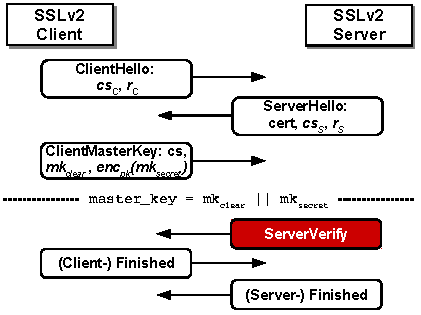
\includegraphics[width=\linewidth]{\DrownFigures/ssl-handshake} 
	\caption{\textbf{\ssltwo handshake.} The server responds with a \texttt{ServerVerify} message directly after receiving an RSA-\PKCS ciphertext contained in \texttt{ClientMasterKey}. This protocol feature enables our attack.\looseness=-1}
	\label{fig:ssl-handshake}
\end{figure}
%\fi
%
A client initiates an \ssltwo handshake by sending a
\texttt{ClientHello} message, which includes a list of cipher
suites $cs_c$ supported by the client and a client nonce $r_c$,
termed \texttt{challenge}.
The server responds with a \texttt{ServerHello} message, which
contains a list of cipher suites $cs_s$ supported by the server,
the server certificate, and a server nonce $r_s$, termed
$\texttt{connection\_ID}$.

The client responds with a \texttt{ClientMasterKey} message, which
specifies a cipher suite supported by both peers and key data
used for constructing a \texttt{master\_key}. In order to support
\textit{export} cipher suites with 40-bit security (e.g.,
\texttt{SSL\_RC2\_128\_CBC\_EXPORT40\_WITH\_MD5}), the key data is
divided into two parts:
\begin{itemize}
	\item $mk_{clear}$: A portion of the \texttt{master\_key} sent in the \texttt{ClientMasterKey} message as plaintext (termed \texttt{clear\_key\_data} in the \ssltwo standard).
	\item $mk_{secret}$: A secret portion of the
          \texttt{master\_key}, encrypted with RSA \PKCS (termed \texttt{secret\_key\_data}). 
\end{itemize}
The resulting \texttt{master\_key} $mk$ is constructed by
concatenating these two keys: $mk = mk_{clear} || mk_{secret}$. For
40-bit export cipher suites, $mk_{secret}$ is five bytes in length.
For non-export cipher suites, the whole \texttt{master\_key} is
encrypted, and the length of $mk_{clear}$ is zero.

The client and server can then compute session keys from the reconstructed \texttt{master\_key} $mk$:

\vspace{-6pt}
\begin{center}
\begin{math}
	\texttt{server\_write\_key} = MD5(mk || ``0" || r_c || r_s) \linebreak	
	\texttt{client\_write\_key} = MD5(mk || ``1" || r_c || r_s)
\end{math}
\end{center}
\vspace{-6pt}

The server responds with a \texttt{ServerVerify} message
consisting of the \texttt{challenge} $r_c$ encrypted with the
\texttt{server\_write\_key}.  Both peers then exchange
\texttt{Finished} messages in order to authenticate to each other.

Our attack exploits the fact that the server always decrypts an RSA-\PKCS
ciphertext, computes the \texttt{server\_write\_key}, and \textit{immediately}
responds with a \texttt{ServerVerify} message.  The \ssltwo standard
implies this message ordering, but does not make it explicit.
However, we observed this behavior in every implementation we
examined.  Our attack also takes advantage of the fact that the
encrypted $mk_{secret}$ portion of the \texttt{master\_key} can vary
in length, and is only five bytes for export ciphers.

% I Merged SSLv2 description and key derivation, ther were some redundancies ...

%\subsubsection{The SSLv2 key derivation mechanism}
%
%Recall that the RSA decryption code on the server decrypts the received RSA ciphertext, and checks the validity of the resulting plaintext as per the PKCS \#1 format. If the plaintext is valid, the server extracts from it the unpadded data, and uses that data, along with other information exchanged thus far during the protocol run, as the key for the chosen symmetric cipher. More formally:
%
%\begin{itemize}
%	\item Let the data from the decrypted RSA plaintext, after padding is removed, be termed \texttt{secret\_key\_data}.
%	\item Recall that the client and server have already exchanged a client nonce, termed \texttt{challenge} in the protocol standard, and a server nonce, termed $\texttt{connection\_ID}$.
%	\item Assume, as is the case throughout this work, that the chosen symmetric cipher is either export RC4 with a 128-bit key, of which 40 bits are secret, or export RC2 with the same key sizes\footnote{details vary slightly, but are very similar for other ciphers}. Then the client should send, along with the RSA ciphertext, a portion of the symmetric key in cleartext, termed \texttt{clear\_key\_data}, where \texttt{clear\_key\_data} is 11 bytes long. The sent \texttt{secret\_key\_data} should be exactly 5 bytes long. Let $\texttt{master\_key} = \texttt{clear\_key\_data} | \texttt{secret\_key\_data}$, where in this context $|$ refers to the concatenation operator.
%	\item Now let
%
%$\texttt{server\_write\_key} = MD5(\texttt{master\_key} | "0" | \texttt{challenge} | \texttt{connection\_ID})$
%
%$\texttt{client\_write\_key} = MD5(\texttt{master\_key} | "1" | \texttt{challenge} | \texttt{connection\_ID})$
%
%where the $|$ operator again means concatenation, and "0" and "1" refer to the corresponding ascii characters.
%
%	\item The respective keys are then used by each party both as keys for the chosen symmetric cipher, and as MAC keys.
%\end{itemize}

%As was hinted in the previous subsection, once an RSA key exchange with PKCS \#1 is implemented, the question immediately arises of how to act given an invalid RSA plaintext - recall that any observable difference in the treatment of invalid messages exposes a Bleichenbacher oracle to the attacker.
%Most implementations, including openssl, employ a counter-mechanism that has become somewhat standard: If the RSA plaintext is invalid or is of a wrong length, generate a random sequence of bytes of the expected length, and treat that sequence of bytes as if that was the plaintext after padding removal.
%
%As an aside, we note this counter-mechanism entails the risk of a timing attack: If the random byte sequence generation takes a measurable amount of time, an attacker may be able to observe the difference in processing times, and deduce the validity of the plaintext. Therefore, this counter-mechanism should be carefully implemented so as to require constant processing time. This is usually done by generating the random byte sequence before the RSA decryption, and choosing between the random sequence and the RSA plaintext according to the validity of the PKCS \#1 formatting. In fact, openssl's implementation of this mechanism was originally not constant-time for SSLv2, but the implementation was appropriately changed after we drew the maintainers' attention to this problem.



\ifsubmit\relax\else
\begin{figure}
	%\centering 
	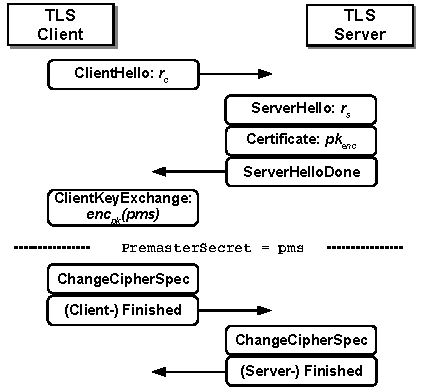
\includegraphics[width=\linewidth]{\DrownFigures/tls-handshake} 
	\caption{\textbf{TLS-RSA handshake.} After receiving an encrypted \pms, the server waits for an authenticated \texttt{ClientFinished} message.}
	\label{fig:tls-handshake}
\end{figure}
\fi

\paragraph{The TLS handshake protocol.}
In TLS~\cite{rfc5246} or \sslthree, the client initiates the handshake with a \texttt{ClientHello}, which contains a client random $r_c$ and a list of supported cipher suites. The server chooses one of the cipher suites and responds with three messages, \texttt{ServerHello}, \texttt{Certificate}, and \texttt{ServerHelloDone}. These messages include the server's choice of cipher suite, server nonce $r_s$, and a server certificate with an RSA public key. The client then uses the public key to encrypt a newly generated 48-byte \pms $pms$ and sends it to the server in a \texttt{ClientKeyExchange} message. The client and server then derive encryption and MAC keys from the \pms and the client and server random nonces. The details of this derivation are not important to our attack.  The client then sends \texttt{ChangeCipherSpec} and \texttt{Finished} messages. The \texttt{Finished} message authenticates all previous handshake messages using the derived keys. The server responds with its own \texttt{ChangeCipherSpec} and \texttt{Finished} messages.

The two main details relevant to our attacks are:
\begin{itemize}
	\item The \pms is always 48 bytes long, independent of the chosen cipher suite.  This is also true for export cipher suites.
	\item After receiving the \texttt{ClientKeyExchange} message, the server waits for the \texttt{ClientFinished} message, in order to authenticate the client.
\end{itemize}


\ifsubmit\relax\else
\subsubsection{Real-world protocol support}
TLSv1.0 is the most commonly supported protocol version, according to several surveys.  The SSL Labs SSL Pulse survey~\cite{ssllabs} reports that 98.6\% of about 140,000 popular TLS/SSL-enabled web sites supported TLSv1.0 in January 2016.  72.0\% supported TLSv1.2.  Support for \ssltwo was at 9.3\%, and \sslthree was at 29\%. Mayer et al.~\cite{DBLP:journals/corr/MayerZSH15} performed Internet-wide surveys of SMTP, IMAP, and POP3 between April and August 2015, and found that support for \ssltwo support was as high as 41.7\% of servers for SMTP on port 25 and as low as 3.7\% of IMAP servers on port 143.  Support for TLSv1.0 was nearly universal on these ports, varying from 91.6\% on port 25 to 98.9\% on port 143.

Bowen~\cite{bowencab} collected 213 million SSL/TLS client hellos and user agent strings from connections to popular sites, of which 183,000 (0.09\%) client hellos supported \ssltwo.  All of these client hellos also supported at least TLSv1.0.

Holz et al.~\cite{2016holz_analysis_tls-based_protocols_electronic_communication} performed passive monitoring to collect information about 16 million SSL/TLS connections during one week in July-August 2015.  They did not report any numbers for \ssltwo, and stated in personal communication that they did not observe any \ssltwo connections in their dataset.
\fi

%In response to our disclosure, OpenSSL has disabled \ssltwo by default in the 1.0.1r and 1.0.2f releases~\cite{opensslchangelog}.  

%This bug was also fixed in the aforementioned openssl releases.

\subsection{Bleichenbacher's attack}
\label{sec:bleichenbacher}
Bleichenbacher's attack is a padding oracle attack---it exploits the
fact that RSA ciphertexts should decrypt to \PKCS-compliant plaintexts.
If an implementation receives an RSA
ciphertext that decrypts to an invalid \PKCS plaintext, it might
naturally leak this information via an error message, by closing the
connection, or by taking longer to process the error condition.  This
behavior can leak information about the plaintext that can be modeled
as a cryptographic \textit{oracle} for the decryption
process. Bleichenbacher~\cite{Bleichenbacher} demonstrated how such an
oracle could be exploited to decrypt RSA ciphertexts.

%For example, the decrypting code may require different processing times for valid vs.\ invalid plaintexts - this is termed a "timing side-channel vulnerability". As another example, the decrypting code may send messages derived in some way from the plaintexts - this is termed a "direct message side channel vulnerability".
%The seminal work in this area \cite{Bleichenbacher} identified the general potential for such vulnerabilities, specifically using a direct message side channel vulnerability present in TLS implementations at the time, and demonstrated how such information could be gradually combined to eventually decrypt the RSA ciphertext in full.

\paragraph{Algorithm.}
In the simplest attack scenario, the attacker has a valid \PKCS
ciphertext $c_{0}$ that they wish to decrypt to discover the message
$m_{0}$.  They have no access to the private RSA key, but instead have
access to an oracle $\Oracle$ that will decrypt a ciphertext $c$ and
inform the attacker whether the most significant two bytes match
the required value for a correct \PKCS padding:
\begin{equation*} 
\Oracle(c) =  
\begin{cases} 
1 & \text{ if } m=c^d \bmod N \text{ starts with \hexb{00}{02}} \\ 
0 & \text{ otherwise.} 
\end{cases} 
\end{equation*} 

If the oracle answers with \texttt{1}, the attacker knows that $2B
\leq m \leq 3B-1$, where $B = 2^{8(\ell_m-2)}$.  The attacker can
take advantage of RSA malleability to generate new candidate ciphertexts
for any $s$:
\[
c = (c_{0} \cdot s^e) \bmod N = (m_{0} \cdot s)^e \bmod N 
\]
The attacker queries the oracle with $c$. If the oracle responds with
$0$, the attacker increments $s$ and repeats the previous
step. Otherwise, the attacker learns that for some~$r$, $2B \leq m_{0}s - rN  < 3B$. This allows the attacker to reduce the range of possible solutions to:  
\[ 
\frac{2B+rN}{s} \leq m_{0} < \frac{3B+rN}{s}  
\] 
The attacker proceeds by refining guesses for $s$ and $r$ values and
successively decreasing the size of the interval containing $m_{0}$.  At
some point the interval will contain a single valid value, $m_{0}$.
Bleichenbacher's original paper describes this process in further
detail~\cite{Bleichenbacher}.

\paragraph{Countermeasures.}
In order to protect against this attack, the decrypter must not leak
information about the \PKCS validity of the ciphertext.  The
ciphertext does not decrypt to a valid message, so the
decrypter generates a fake plaintext and continues the
protocol with this decoy.  The attacker should not be able to
distinguish the resulting computation from a correctly decrypted
ciphertext.

In the case of SSL/TLS, the server generates a random \pms to continue
the handshake if the decrypted ciphertext is
invalid.  The client will not possess the session key to send a valid
\texttt{ClientFinished} message and the connection will terminate.



%\input{libraries}

% !TEX root = subgroup.tex
\ApplicationsTable

\section{TLS}\label{sec:tls}

TLS (Transport Layer Security) is a transport layer protocol designed to provide confidentiality,
integrity and (most commonly) one-side authentication for application sessions. 
It is widely used to protect HTTP and mail protocols. 

A TLS client initiates a TLS handshake with the \texttt{Client\-Hello} message.
This message includes a list of supported cipher suites, and a client random
nonce $r_c$. The server responds with a \texttt{Server\-Hello} message containing
the chosen cipher suite and server random nonce $r_s$, and a
\texttt{Certificate} message that includes the server's X.509 certificate. If
the server selects a cipher suite using ephemeral Diffie-Hellman key exchange,
the server additionally sends a \texttt{Server\-Key\-Exchange} message containing
the server's choice of Diffie-Hellman parameters $p$ and $g$, the server's
Diffie-Hellman public value $y_s = g^{x_s} \bmod p$, a signature by the
server's private key over both the client and server nonces ($r_c$ and $r_s$),
and the server's Diffie-Hellman parameters ($p$, $g$, and $y_s$). The client
then verifies the signature using the public key from the server's certificate,
and responds with a \texttt{Client\-Key\-Exchange} message containing the client's
Diffie-Hellman public value $y_c = g^{x_c} \bmod p$. The Diffie-Hellman shared
secret $Y = g^{x_s x_c} \bmod p$ is used to derive encryption and MAC keys. The
client then sends \texttt{Change\-Cipher\-Spec} and \texttt{Finished} messages. The
\texttt{Finished} message contains a hash of the handshake transcript, and is
encrypted and authenticated using the derived encryption and MAC keys. Upon
decrypting and authenticating this message, the server verifies that the hash
of the transcript matches the expected hash.  Provided the hash matches, the
server then sends its own \texttt{Change\-Cipher\-Spec} and \texttt{Finished}
messages, which the client then verifies. If either side fails to decrypt or
authenticate the \texttt{Finished} messages, or if the transcript hashes do not
match, the connection fails immediately~\cite{rfc5246}.

TLS also specifies a mode of using Diffie-Hellman with fixed parameters from
the server's certificate~\cite{rfc3279}. This mode is not forward secret, was
never widely adopted, and has been removed from all modern browsers due to
dangerous protocol flaws~\cite{kci-tls-2015}. The only widely used form of
Diffie-Hellman in TLS today is ephemeral Diffie-Hellman, described above.

\subsection{Small Subgroup Attacks in TLS}
\label{sec:tls-subgroup-attack}

\paragraph{Small subgroup confinement attacks}
A malicious TLS server can perform a variant of the small subgroup attack
against a client by selecting group parameters $g$ and $p$ such that $g$
generates an insecure group order. TLS versions prior to 1.3 give the server
complete liberty to choose the group, and they do not include any method for
the server to specify the desired group order $q$ to the client.  This means a
client has no feasible way to validate that the group sent by the server has the
desired level of security or that a server's key exchange value is in
the correct group for a non-safe prime.
\looseness=-1

Similarly, a man in the middle with knowledge of the server's long-term private
signing key can use a small subgroup confinement attack to more easily
compromise perfect forward secrecy, without having to rewrite an entire
connection. The attack is similar to the those described by Bhargavan and
Delignat-Lavaud~\cite{bhargavan-channel-bindings-2015}. The attacker modifies the
server key exchange message, leaving the prime unchanged, but substituting a
generator $g_i$ of a subgroup of small order $q_i$ for the group generator and 
$g_i$ for the server's key exchange value $y_s$. The attacker then forges a correct signature for the modified server key exchange message and passes it to the client.  The client then
responds with a client key exchange message $y_c = g_i^{x_c} \bmod p$, which
the man-in-the-middle leaves unchanged. The server's view of the shared secret
is then $g_i^{x_c x_s} \bmod p$, and the client's view of the shared secret is
$g_i^{x_c} \bmod p$. These views are identical when ${x_s} \equiv 1 \bmod q_i$,
so this connection will succeed with probability $1/q_i$. For small enough
$q_i$, this enables a man in the middle to use a compromised server signing key to
decrypt traffic from forward-secret ciphersuites with a reasonable probability
of success, while only requiring tampering with a single handshake message,
rather than having to actively rewrite the entire connection for the duration of the session.

Furthermore, if the server uses a static Diffie-Hellman key exchange value,
then the attacker can perform a small subgroup key-recovery attack as the
client in order to learn the server's static exponent $x_s \bmod q_i$ for the
small subgroup. This enables the attacker to calculate a custom generator such
that the client and server views of the shared secret are always identical,
raising the above attack to a 100\% probability of success.

\TLSLibraryTable

\paragraph{Small subgroup key recovery attacks} In TLS, the client must
authenticate the handshake before the server, by providing a valid
\texttt{Finished} message. This forces a small subgroup key recovery attack
against TLS to be primarily online. To perform a Lim-Lee small subgroup key
recovery attack against a server static exponent, a malicious client initiates
a TLS handshake and sends a generator $g_i$ of a small subgroup of order $q_i$
as its client key exchange message $y_c$.  The server will calculate $Y_s =
g_i^{x_s} \bmod p$ as the shared secret. The server's view of the shared secret
is confined to the subgroup of order $q_i$.  However, since $g_i$ and $g$
generate separate subgroups, the server's public value $y_s = g^x_s$ gives the
attacker no information about the value of the shared secret $Y_s$. Instead,
the attacker must guess a value for $x_s \bmod q_i$, and send the corresponding
client \texttt{Finished} message. If the server continues the handshake, the
attacker learns that the guess is correct.  Therefore, assuming the server is
reusing a static value for $x_s$, the attacker needs to perform at most $q_i$
queries to learn the  server's secret $x_s \bmod q_i$~\cite{lim-1997}. This
attack is feasible if $q_i$ is small enough and the server reuses
Diffie-Hellman exponents for sufficiently many requests.

The attacker repeats this process for many different primes $q_i$, and uses the
Chinese remainder theorem to combine them modulo the product of the primes
$q_i$.  The attacker can also use the Pollard lambda algorithm to reconstruct
any remaining bits of the exponent~\cite{lim-1997}.



We note that the TLS False Start extension allows the
server to send application data before receiving the client's authentication~\cite{rfc7918}.
The specification only allows this behavior for abbreviated handshakes, which
do not include a full key exchange.  If a full key exchange were allowed, the
fact that the server authenticates first would allow a malicious client to
mount a mostly offline key recovery attack.
%\todo{Add discussion of the old unused TLS extension that makes this offline. \ref{rfc7918}}



\subsection{OpenSSL}

Prior to early 2015, OpenSSL defaulted to using static-ephemeral Diffie-Hellman
values. Server applications generate a fresh Diffie-Hellman secret exponent on
startup, and reuse this exponent until they are restarted.  A server would be
vulnerable to small subgroup attacks if it chose a DSA prime, explicitly
configured the \texttt{dh->length} parameter to generate a short exponent, and
failed to set \texttt{SSL\_OP\_SINGLE\_DH\_USE} to prevent repeated exponents.
OpenSSL provides some test code for key generation which configures DSA group
parameters, sets an exponent length to the group order, and correctly sets the
\texttt{SSL\_OP\_SINGLE\_DH\_USE} to generate new exponents on every
connection.  We found this test code widely used across many applications.  We
discovered that Unbound, a DNS resolver, used the same parameters as the tests,
but without setting \texttt{SSL\_OP\_SINGLE\_DH\_USE}, rendering them
vulnerable to a key recovery attack.  A number of other applications including
Lighttpd used the same or similar code with non-safe primes, but correctly set
\texttt{SSL\_OP\_SINGLE\_DH\_USE}.

In spring 2015, OpenSSL added explicit support for RFC~5114
groups~\cite{openssl-changelog-102}, including the ability for servers to
specify a subgroup order in a set of Diffie-Hellman group parameters. When the
subgroup order is specified, the exponent length is automatically adjusted to
match the subgroup size.  However, the update did not contain code to validate
subgroup order for key exchange values, leaving OpenSSL users vulnerable to
precisely the key recovery attack outlined in
Section~\ref{sec:tls-subgroup-attack}.

We disclosed this vulnerability to OpenSSL in January 2016. The vulnerability
was patched by including code to validate subgroup order when a subgroup was
specified in a set of Diffie-Hellman parameters and setting
\texttt{SSL\_OP\_SINGLE\_DH\_USE} by default~\cite{openssl-secadv-subgroup}.
Prior to this patch, any code using OpenSSL for DSA-style Diffie-Hellman
parameters was vulnerable to small subgroup attacks by default.

Exim~\cite{exim}, a popular mail server that uses OpenSSL, provides a clear
example of the fragile situation created by this update. By default, Exim uses
the RFC~5114 Group 23 parameters with OpenSSL, does not set an exponent length,
and does not set \texttt{SSL\_OP\_SINGLE\-\_DH\_USE}. In a blog post, an Exim
developer explains that because of ``numerous issues with automatic generation
of DH parameters'', they added support for fixed groups specified in RFCs and picked
Group~23 as the default~\cite{exim-blog}.  Exim narrowly avoided being fully
vulnerable to a key recovery attack by not including the size of the subgroup
generated by $q$ in the Diffie-Hellman parameters that it passes to OpenSSL.
Had this been included, OpenSSL would have automatically shortened the exponent
length, leaving the server fully vulnerable to a key recovery attack.  For this
group, an attacker can recover 130 bits of information about the secret
exponent using $2^{33}$ online queries, but this does not allow the attacker to
recover the server's 2048-bit exponent modulo the correct 224-bit group order
$q$ as the small subgroup orders $q_i$ are all relatively prime to $q$.

We looked at several other applications as well, but did not find them to be
vulnerable to key recovery attacks (Table~\ref{tab:common-applications}).



% comprising 53.62\% of all such servers~\cite{esoft2016}.

% Exim can be compiled either with GNU TLS or with OpenSSL. When compiled with OpenSSL,
% it supports single use DH keys with an option that is off by default
% (as of version 4.87, the latest at time of writing). In OpenSSL mode, it
% includes checks for unsafe primes and incorrect generators, however it
% ignores the generator check when the generator is not 2 or 5, due to a known
% bug in OpenSSL. More significantly, it utilizes the DSA primes with small
% subgroups. Their code comments note ``These have been thoroughly reviewed as
% meeting certain eligibility criteria, which is more than can be said for primes
% generated quickly''. However, they fail to note the difference in criteria for
% the DSA primes as opposed to the others, resulting in the selection of vulnerable
% groups. The subgroup size $q$ was not included in the Exim's default DSA parameter, saving 
% a default Exim installation from being vulnerable to the attack described 
% in Section~\ref{sec:tls-subgroup-attack} due the fact that OpenSSL did not have the possibility 
% to match the exponent length to subgroup size. Said that, if the DSA parameter would have been generated using the 
% OpenSSL's genpkey utility~\cite{genpkey} all the conditions to perform the Small subgroup key recovery attack
% as per Section ~\ref{sec:tls-subgroup-attack} would have been met.
% In comparison Postfix an MX  utilized for 32.80\% of mail servers~\cite{esoft2016}
% suggests generating a group at install time but neglects to set the single use OpenSSL option
% and includes two hardcoded groups by default.



\ScanTable

\subsection{Other Implementations} \label{subsec:nss}

We examined the source code of multiple TLS implementations
(Table~\ref{tab:tls-implementations}). Prior to January 2016, no TLS
implementations that we examined validated group order, even for the well-known
DSA primes from RFC~5114, leaving them vulnerable to small subgroup confinement attacks.

Most of the implementations we examined attempt to match exponent length to the
perceived strength of the prime. For example, Mozilla Network Security Services
(NSS), the TLS library used in the Firefox browser and some versions of
Chrome~\cite{nss-overview,chrome-to-openssl}, uses NIST's ``comparable key strength'' recommendations
on key management~\cite{sp800} to determine secret exponent lengths from the length of the prime.~\cite{nss-line-of-code}  Thus NSS uses 160-bit exponents with a 1024-bit prime, and 224-bit exponents with a 2048-bit prime.
 In fall 2015, NSS added an additional check to ensure that the
shared secret $g^{x_ax_b} \not \equiv 1 \bmod p$~\cite{nss-code-secret-not-one}.

Several implementations go to elaborate lengths to match exponent length to
perceived prime strength.  The Cryptlib library fits a quadratic curve to the
small exponent attack cost table in the original van~Oorschot
paper~\cite{van1996diffie} and uses the fitted curve to determine safe key
lengths~\cite{cryptlib-fitted-curve}. The Crypto++ library uses an explicit
``work factor'' calculation, evaluating the function $2.4 n^{1/3} (\log
n)^{2/3}$~\cite{cryptoplusplus-work-factor}. Subgroup order and exponent
lengths are set to twice the calculated work factor. The work factor
calculation is taken from a 1995 paper by Odlyzko on integer
factorization~\cite{odlyzko-1995}. Botan, a C++ cryptography and TLS library,
uses a similar work factor calculation, derived from RFC~3766~\cite{rfc3766},
which describes best practices as of 2004 for selecting public key strengths
when exchanging symmetric keys. RFC~3766 uses a similar work factor algorithm
to Odlyzko, intended to model the running time of the number-field
sieve. Botan then doubles the length of the work factor to obtain subgroup and
exponent lengths~\cite{botan-double}.

% Apple Safari on OS X and iOS performed no validation of
% Diffie-Hellman prime lengths until July 2015, and supported connections where
% the server offered a trivially-broken group using a 16-bit prime~\cite{weakdh-ccs15}.

\subsection{Measurements}
\label{sec:tls-measurements}

We used ZMap~\cite{zmap-2013} to probe the public IPv4 address space for hosts
serving three TLS-based protocols: HTTPS, SMTP+STARTTLS, and POP3S\@.  To
determine which primes servers were using, we sent a \texttt{ClientHello}
message containing only ephemeral Diffie-Hellman cipher suites.  We combined
this data with scans from Censys~\cite{censys} to determine the overall
population.  The results are summarized in Table~\ref{tab:scandata}. 

\TLSHostValidationTable

\PrimesAllTLS

In August 2016, we conducted additional scans of a random 1\% sample
of HTTPS hosts on the Internet.  First, we checked for nontrivial
small subgroup attack vulnerability. For servers that sent us a prime
$p$ such that $p-1$ was divisible by 7, we attempted a handshake using
a client key exchange value of $g_7\bmod p$, where $g_7$ is a
generator of a subgroup of order $7$.  (7 is the smallest prime factor
of $p-1$ for Group 22.) When we send $g_7$, we expect to correctly
guess the \texttt{PreMasterSecret} and complete the handshake with one
seventh of hosts that do not validate subgroup order. In our scan, we
were able to successfully complete a handshake with $1477$ of $10714$
hosts that offered a prime such that $p-1$ was divisible by $7$,
implying that approximately 96\% of these hosts fail to validate
subgroup order six months after OpenSSL pushed a patch adding group
order validation for correctly configured groups.

Second, we measured how many hosts performed even the most basic
validation of key exchange values. We attempted to connect to HTTPS hosts with
the client key exchange values of $y_c = 0 \bmod p, 1 \bmod p, -1 \bmod p$. As
Table~\ref{tab:tlsvalidation} shows, we found that over 5\% of hosts that
accepted DHE ciphersuites accepted the key exchange value of $-1 \bmod p$ and
derived the \texttt{PreMasterSecret} from it. These implementations are
vulnerable to a trivial version of the small subgroup confinement attacks
described in Section~\ref{sec:tls-subgroup-attack}, for \emph{any} prime
modulus $p$. By examining the default web pages of many of these hosts,
we identified products from several notable companies including Microsoft,
Cisco, and VMWare. When we disclosed these findings, VMWare notified us that
they had already applied the fix in the latest version of their products;
Microsoft acknowledged the missing checks but chose not to include them since
they only use safe primes, and adding the checks may break functionality
for some clients that were sending unusual key exchange values; and Cisco
informed us that they would investigate the issue.

Of 40.6\,M total HTTPS hosts found in our scans, 10.8\,M~(27\%) supported
ephemeral Diffie-Hellman, of which 1.6\,M~(4\%) used a non-safe prime, and
309\,K~(0.8\%) used a non-safe prime and reused exponents across multiple
connections, making them likely candidates for a small subgroup key recovery
attack.  We note that the numbers for hosts reusing exponents are an
underestimate, since we only mark hosts as such if we found them using the same
public Diffie-Hellman value across multiple connections, and some load
balancers that cycle among multiple values might have evaded detection.

While 77\%~of POP3S hosts and 39\%~of SMTP servers used a non-safe prime, a
much smaller number used a non-safe prime and reused exponents (<0.01\% in both
protocols), suggesting that the popular implementations (Postfix and
Dovecot~\cite{mail-2015}) that use these primes follow recommendations to use
ephemeral Diffie-Hellman values with DSA primes.

Table~\ref{tab:primes} shows nine groups that accounted for the majority of
non-safe primes used by hosts in the wild. Over 1.17\,M hosts across all of our
HTTPS scans negotiated Group~22 in a key exchange. To get a better picture of
which implementations provide support for this group, we examined the default
web pages of these hosts to identify companies and products, which we show in
Table~\ref{tab:tls-group22-support}.

\TLSGroupSupport


Of the the 307\,K HTTPS hosts that both use non-safe primes and reuse
exponents, 277\,K~(90\%) belong to hosts behind Amazon's Elastic Load
Balancer~\cite{amazon-elb}. These hosts use a 1024-bit prime with a 160-bit
subgroup. We set up our own load balancer instance and found that the
implementation failed to validate subgroup order. We were able to use a
small-subgroup key recovery attack to compute 17 bits of our load balancer's
private Diffie-Hellman exponent $x_s$ in only 3813 queries.  We responsibly
disclosed this vulnerability to Amazon. Amazon informed us that they have
removed Diffie-Hellman from their recommended ELB security policy, and are
encouraging customers to use the latest policy.  In May 2016, we performed
additional scans and found that 88\% of hosts using this prime no longer
repeated exponents.   We give a partial factorization for $p-1$ in
Table~\ref{tab:group-order-factorization}; the next largest subgroups have 61
and 89 bits and an offline attack against the remaining bits of a 160-bit
exponent would take $2^{71}$ time.  For more details on the computation, see
Section~\ref{sec:ecm}.

SSLeay~\cite{ssleay}, a predecessor for OpenSSL, includes several default
Diffie-Hellman primes, including a 512-bit prime. We found that 717 SMTP
servers used a version of the OpenSSL 512-bit prime with a single character
difference in the hexadecimal representation.  The resulting modulus that these
servers use for their Diffie-Hellman key exchange is no longer prime. We
include the factorization of this modulus along with the factors of the
resulting group order in Table~\ref{tab:group-order-factorization}. The use of
a composite modulus further decreases the work required to perform a small
subgroup attack.

Although TLS also includes static Diffie-Hellman cipher suites that require a
DSS certificate, we did not include them in our study; no browser supports
static Diffie-Hellman~\cite{kci-tls-2015}, and Censys shows no hosts with DSS
certificates, with only 652 total hosts with non-RSA or ECDSA certificates.

%In February 2016, we conducted an additional scan of a random 1\% sample of the
%Internet to check how many hosts performed even the most basic validation of
%key exchange values. We attempted to connect to HTTPS hosts with a client
%key exchange message of $y_c = 1$. We found that 322 of 589,241 hosts accepted
%this key exchange value and derived the \texttt{PreMasterSecret} from it. 248
%of these hosts were Cisco devices, another 28 were VMware Horizon View servers,
%and the remaining 46 devices did not fit into any clear category. These
%implementations are vulnerable to a trivial version of the small subgroup
%confinement attacks described in Section~\ref{sec:tls-subgroup-attack}.\todo{did we disclose this? we need to. also what about validation of values other than 0?}


%\TODO{classify implementations again and disclose to Cisco, etc}








% !TEX root = ../../../proposal.tex

\section{IPsec}

%Description of IKEv1 and IKEv2.

IPsec is a set of Layer-3 protocols which add confidentiality, data protection,
sender authentication, and access control to IP traffic. IPsec is commonly used
to implement VPNs.
%IPsec provides two types of security service: Authentication Header (AH),
%which provides sender authentication, and Encapsulating Security Payload
%(ESP), which provides both sender authentication and payload encryption.  Each
%of these services requires the communicating parties to establish shared
%state, which includes the cryptographic algorithms used to provide the service
%and the keys used as input for the cryptographic algorithms.
IPsec uses the Internet Key Exchange (IKE) protocol to determine the keys used
to secure a session. IPsec may use IKEv1~\cite{rfc2409} or
IKEv2~\cite{rfc7296}. While IKEv2 is not backwards-compatible with IKEv1, the
two protocols are similar in message structure and purpose. Both versions use
Diffie-Hellman to negotiate shared secrets. The groups used are limited to a
fixed set of pre-determined choices, which include the DSA groups from
RFC~5114, each assigned a number by IANA~\cite{rfc3526,rfc5114,rfc7296}.

% IKE versions
\paragraph{IKEv1}
%IKEv1 is a hybrid protocol built upon three other protocols:
%ISAKMP~\cite{rfc2408}, which establishes a framework for authentication and
%key exchange; Oakley~\cite{rfc2412}, which defines a series of key exchanges
%and services based on the Diffie-Hellman key exchange; and
%SKEME~\cite{krawczyk1996skeme}, a key exchange protocol that provides
%anonymity, repudiability, and quick key refreshement.  IKEv1 is formally
%defined in RFCs 2407~\cite{rfc2407}, 2408~\cite{rfc2408}, and
%2409~\cite{rfc2409}. 
IKEv1~\cite{rfc2407,rfc2408,rfc2409} has two basic methods for authenticated
key exchange: Main Mode and Aggressive Mode. Main Mode requires six messages to
establish the requisite state. The initiator sends a Security Association
(\texttt{SA}) payload, containing a selection of cipher suites and
Diffie-Hellman groups they are willing to negotiate. The responder selects a
cipher and responds with its own \texttt{SA} payload. After the cipher suite is
selected, the initiator and responder both transmit Key Exchange (\texttt{KE})
payloads containing public Diffie-Hellman values for the chosen group. At this
point, both parties compute shared key materials, denoted \texttt{SKEYID}. When
using signatures for authentication, \texttt{SKEYID} is computed
$\texttt{SKEYID} = \operatorname{prf}(N_i | N_r, g^{x_ix_r})$.  For the other
two authentication modes, pre-shared key and public-key encryption,
\texttt{SKEYID} is derived from the pre-shared key and session cookies,
respectively, and does not depend on the negotiated Diffie-Hellman shared
secret.

Each party then in turn sends an authentication message (\texttt{AUTH}) derived
from a hash over \texttt{SKEYID} and the handshake. The authentication messages
are encrypted and authenticated using keys derived from the Diffie-Hellman
secret $g^{x_i x_r}$.  The responder only sends her \texttt{AUTH} message after
receiving and validating the initiator's \texttt{AUTH} message.

Aggressive Mode operates identically to Main Mode, but in order to reduce
latency, the initiator sends \texttt{SA} and \texttt{KE} messages together, and
the responder replies with its \texttt{SA}, \texttt{KE}, and \texttt{AUTH}
messages together. In aggressive mode, the responder sends an authentication
message first, and the authentication messages are not encrypted.


\paragraph{IKEv2}
%IKE Version 2 (IKEv2) was released in RFC 4306~\cite{rfc4306} to replace IKEv1
%and the plethora of RFCs that define it. RFC 7296~\cite{rfc7296} gives the
%current version of the IKEv2 specification.
IKEv2~\cite{rfc4306,rfc7296} combines the \texttt{SA} and \texttt{KE} messages
into a single message. The initiator provides a best guess ciphersuite for the
\texttt{KE} message. If the responder accepts that proposal and chooses not to
renegotiate, the responder replies with a single message containing both
\texttt{SA} and \texttt{KE} payloads. Both parties then send and verify
\texttt{AUTH} messages, starting with the initiator.  The authentication
messages are encrypted using session keys derived from the \texttt{SKEYSEED}
value which is derived from the negotiated Diffie-Hellman shared secret. The
standard authentication modes use public-key signatures over the handshake
values.

%IKE Group~23, the 2048-bit MODP group with a 224-bit subgroup, is particularly
%vulnerable as shown in Section~\ref{sec:ecm}.

\subsection{Small Subgroup Attacks in IPsec} There are several variants of
small subgroup attacks against IKEv1 and IKEv2.  We describe the attacks
against these protocols together in this section.

\paragraph{Small subgroup confinement attacks} First, consider attacks that can
be carried out by an attacking initiator or responder. In IKEv1 Main Mode and
in IKEv2, either peer can carry out a small subgroup confinement attack against
the other by sending a generator of a small subgroup as its key exchange value.
The attacking peer must then guess the other peer's view of the Diffie-Hellman
shared secret to compute the session keys to encrypt its authentication
message, leading to a mostly online attack. However, in IKEv1 Aggressive Mode,
the responder sends its \texttt{AUTH} message before the initiator, and this
value is not encrypted with a session key. If signature authentication is being
used, the \texttt{SKEYID} and resulting hashes are derived from the
Diffie-Hellman shared secret, so the initiator can perform an offline
brute-force attack against the responder's authentication message to learn
their exponent in the small subgroup.

Now, consider a man-in-the-middle attacker. Bhargavan, Delignat-Lavaud, and
Pironti~\cite{bhargavan-channel-bindings-2015} describe a transcript synchronization
attack against IKEv2 that relies on a small subgroup confinement attack.  A
man-in-the-middle attacker initiates simultaneous connections with an initiator
and a responder using identical nonces, and sends a generator $g_i$ for a
subgroup of small order $q_i$ to each as its \texttt{KE} message.  The two
sides have a $1/q_i$ chance of negotiating an identical shared secret, so an
authentication method depending only on nonces and shared secrets could be
forwarded, and the session keys would be identical.

If the attacker also has knowledge of the secrets used for authentication, more
attacks are possible.  Similar to the attack described for TLS, such an
attacker can use a small subgroup confinement attack to force a connection to
use weak encryption. The attacker only needs to rewrite a small number of
handshake messages; any further encrypted communications can then be decrypted
at leisure without requiring the man-in-the-middle attacker to continuously
rewrite the connection. We consider a man-in-the-middle attacker who modifies
the key exchange message from both the initiator and the responder to
substitute a generator $g_i$ of a subgroup of small order $q_i$.  The attacker
must then replace the handshake authentication messages, which would require
knowledge of the long-term authentication secret.  We describe this attack for
each of pre-shared key, signatures, and public-key authentication. 

For pre-shared key authentication in IKEv1 Main Mode, IKEv1 Aggressive Mode,
and IKEv2, the man-in-the-middle attacker must only know the pre-shared key to
construct the authentication hash; the authentication message does not depend
on the negotiated Diffie-Hellman shared secret. With probability $1/q_i$, the
two parties will agree on the Diffie-Hellman shared secret. The attacker can
then brute force this value after viewing messages encrypted with keys derived
from it.

For signature authentication in IKEv1 Main Mode and in IKEv2, the signed hash
transmitted from each side is derived from the nonces and the negotiated shared
secret, which is confined to one of $q_i$ possible values.  The attacker must
know the private signing keys for both initiator and responder and brute force
\texttt{SKEYID} from the received signature in order to forge the modified
authentication signatures on each side. The communicating parties will have a
$q_i$ chance of agreeing on the same value for the shared secret to allow the
attack to succeed. For IKEv1 Aggressive Mode, the attack can be made to succeed
every time. The responder's key exchange message is sent together with their
signature which depends on the negotiated shared secret, so the
man-in-the-middle attacker can brute force the $q_i$ possible values of the
responders private key $x_r$ and replace the responder's key exchange message
with $q_i^{x_r}$, forging an appropriate signature with their knowledge of the
signing key.

For public key authentication in IKEv1 Main Mode, IKEv1 Aggressive Mode, and
IKEv2, the attacker must know the private keys corresponding to the public keys
used to encrypt the ID and nonce values on both sides in order to forge a valid
authentication hash.  Since the authentication does not depend on the shared
Diffie-Hellman negotiated value, a man-in-the-middle attacker must then brute
force the negotiated shared key once they receives a message encrypted with the
derived key.  The two parties will agree on their view of the shared key with
probability $1/q_i$, allowing the attack to succeed.

\paragraph{Small subgroup key recovery attacks} Similar to TLS, an IKE
responder that reuses private exponents and does not verify that the initiator
key exchange values are in the correct subgroup is vulnerable to a small
subgroup key recovery attack. The most recent version of the IKEv2
specification has a section discussing reuse of Diffie-Hellman exponents,
and states that ``because computing Diffie-Hellman exponentials is
computationally expensive, an endpoint may find it advantageous to reuse those
exponentials for multiple connection setups''~\cite{rfc7296}. Following this
recommendation could leave a host open to a key recovery attack, depending on
how exponent reuse is implemented. A small subgroup key recovery attack on IKE
would be primarily offline for IKEv1 with signature authentication and for
IKEv2 against the initiator.

For each subgroup of order $q_i$, the attacker's goal is to obtain a responder
\texttt{AUTH} message, which depends on the secret chosen by the responder. If
an \texttt{AUTH} message can be obtained, the attacker can brute-force the
responder's secret within the subgroup offline. This is possible if the server
supports IKEv1 Aggressive Mode, since the server authenticates before the
client, and signature authentication produces a value dependent on the
negotiated secret.  In all other IKE modes, the client authenticates first,
leading to an online attack. The flow of the attack is identical to TLS; for
more details see Section~\ref{sec:tls}.

Ferguson and Schneier~\cite{ferguson2000cryptographic} describe a hypothetical
small-subgroup attack against the initiator where a man-in-the-middle attacker
abuses undefined behavior with respect to UDP packet retransmissions. A
malicious party could ``retransmit'' many key exchange messages to an initiator
and potentially receive a different authentication message in response to each,
allowing a mostly offline key recovery attack.

%The attacker must choose their key exchange value to be a generator of the
%selected subgroup, which we call $g_i$.  When the responder computes the
%shared secret, $g_i^a$, it will lie within the chosen subgroup.  The attacker
%must guess $g_i^a \bmod q_i$, and construct their \texttt{AUTH} message
%accordingly.  The responder will reply with an \texttt{AUTH} message in the
%event of a correct guess, and an error message otherwise.  With repeated
%guessing, the attacker can learn the value of $g_i^a$ for each subgroup, and
%take advantage of the Pollard labmda algorithm to solve for the rest of the
%secret offline within the reduced search space.

\subsection{Implementations}

We examined several open-source IKE implementations to understand server
behavior.  In particular, we looked for implementations that generate small
Diffie-Hellman exponents, repeat exponents across multiple connections, or do
not correctly validate subgroup order. Despite the suggestion in IKEv2 RFC 7296
to reuse exponents~\cite{rfc7296}, none of the implementations that we examined
reused secret exponents. 

% This is already included in the intro
%RFC 6989~\cite{rfc6989} (``Additional Diffie-Hellman Tests for IKEv2'')
%specifies additional checks that IKE implementations supporting MODP groups
%with small subgroups should perform. The RFC requries IKE implementations to
%choose between either checking that the peer's public value is in the correct
%subgroup, or it must never reuse Diffie-Hellman private values. 

All implementations we reviewed are based on FreeS/WAN~\cite{freeswan}, a
reference implementation of IPSec. The final release of FreeS/Wan, version
2.06, was released in 2004. Version 2.04 was forked into
Openswan~\cite{openswan} and strongSwan\cite{strongswan}, with a further fork
of Openswan into Libreswan~\cite{libreswan} in 2012.  The final release of
FreeS/WAN used constant length 256-bit exponents but did not support RFC~5114
DSA groups, offering only the Oakley 1024-bit and 1536-bit groups that use safe
primes.

\IKEGroupSupportAndValidationTable

Openswan does not generate keys with short exponents. By default, RFC~5114
groups are not supported, although there is a compile-time option that can be
explicitly set to enable support for DSA groups.  strongSwan both supports
RFC~5114 groups and has explicit hard-coded exponent sizes for each group. The
exponent size for each of the RFC~5114 DSA groups matches the subgroup size.
However, these exponent sizes are only used if the
\texttt{dh\_exponent\_ansi\_x9\_42} configuration option is set. It also
includes a routine inside an \texttt{\#ifdef} that validates subgroup order by
checking that $g^q \equiv 1 \bmod p$, but validation is not enabled by default.
Libreswan uses Mozilla Network Security Services (NSS)~\cite{nss-overview} to
generate Diffie-Hellman keys. As discussed in Section~\ref{subsec:nss}, NSS
generates short exponents for Diffie-Hellman groups. Libreswan was forked from
Openswan after support for RFC~5114 was added, and retains support for those
groups if it is configured to use them. 

Although none of the implementations we examined were configured to reuse
Diffie-Hellman exponents across connections, the failure to validate subgroup
orders even for the pre-specified groups renders these implementations fragile
to future changes and vulnerable to subgroup confinement attacks.

Several closed source implementations also provide support for RFC~5114
Group~24. These include Cisco's IOS~\cite{ciscogroup24}, Juniper's
Junos~\cite{junosgroup24}, and Windows Server 2012 R2~\cite{windowsgroup24}. We
were unable to examine the source code for these implementations to determine
whether or not they validate subgroup order.

%\IKEGroupSupportAndValidationTable

\subsection{Measurements}

We performed a series of Internet scans using ZMap to identify IKE responders.
In our analysis, we only consider hosts that respond to our ZMap scan probes.
Many IKE hosts that filter their connections based on IP are excluded from our
results.  We further note that, depending on VPN server configurations, some
responders may continue with a negotiation that uses weak parameters until they
are able to identify a configuration for the connecting initiator. At that
point, they might reject the connection. As an unauthenticated initiator, we
have no way of distinguishing this behavior from the behaviour of a VPN server
that legitimately accepts weak parameters. For a more detailed explanation of
possible IKE responder behaviors in response to scanning probes, see
Wouters~\cite{paul-wouters}.

In October 2016, we performed a series of scans offering the most common cipher
suites and group parameters we found in implementations to establish a baseline
population for IKEv1 and IKEv2 responses. For IKEv1, the baseline scan offered
Oakley groups 2 and 14 and RFC~5114 groups 22, 23, and 24 for the group
parameters; SHA1 or SHA256 for the hash function; pre-shared key or RSA
signatures for the authentication method; and AES-CBC, 3DES, and DES for the
encryption algorithm.  Our IKEv2 baseline scan was similar, but also offered
the 256-bit and 384-bit ECP groups and AES-GCM for authenticated encryption.

On top of the baseline scans, we performed additional scans to measure support
for the non-safe RFC~5114 groups and for key exchange parameter validation.
Table~\ref{tab:ikegroupsupportandvalidation} shows the results of the October
IKE scans.  For each RFC~5114 DSA group, we performed four handshakes with each
host; the first tested for support by sending a valid client key exchange
value, and the three others tested values that should be rejected by a
properly-validating host. We did not scan using the key exchange value $0$
because of a vulnerability present in unpatched Libreswan and Openswan
implementations that causes the IKE daemon to restart when it receives such a
value~\cite{cve-2015-3240}.

We considered a host to accept our key exchange value if after receiving the
value, it continued the handshake without any indication of an error. We found
that 33.2\% of IKEv1 hosts and 17.7\% of IKEv2 hosts that responded to our
baseline scans supported using one of the RFC 5114 groups, and that a
surprising number of hosts failed to validate key exchange values.  24.8\% of
IKEv1 hosts that accepted Group 23 with a valid key exchange value also
accepted $1 \bmod p$ or $-1 \bmod p$ as a key exchange value, even though this
is explicitly warned against in the RFC~\cite{rfc2412}.  This behavior leaves
these hosts open to a small subgroup confinement attack even for safe primes,
as described in Section~\ref{subsec:small-subgroup-attack}.

For safe groups, a check that the key exchange value is strictly between $1$
and $p-1$ is sufficient validation. However, when using non-safe DSA primes, it
is also necessary to verify that the key exchange value lies within the correct
subgroup (\ie, $y^q \equiv 1 \bmod p$). To test this case, we constructed a
generator of a subgroup that was not the intended DSA subgroup, and offered
that as our key exchange value. We did not find any IKEv1 hosts that rejected
this key exchange value after previously accepting a valid key exchange value
for the given group. For IKEv2, the results were similar with the exception of
Group 24, where still over 93\% of hosts accepted this key exchange value. This
suggests that almost no hosts supporting DSA groups are correctly validating
subgroup order. 

We observed that across all of the IKE scans, 109 IKEv1 hosts and 52 IKEv2
hosts repeated a key exchange value. This may be due to entropy issues in key
generation rather than static Diffie-Hellman exponents; we also found 15,891
repeated key exchange values across different IP addresses. We found no hosts
that used both repeated key exchange values and non-safe groups. We summarize
these results in Table~\ref{tab:scandata}. 

%The results of these scans are presented in Table~\ref{tab:scandata}.  To get
%a an estimate of the number of hosts that support each IKE version, we
%conducted scans of 1\% of the IPv4 address space using Zmap. If the host
%responded with a valid message for the IKE version we were scanning for, we
%considered it to support that version. The numbers present for IKE support in
%Table~\ref{tab:scandata} are extrapolated from these 1\% scans.

%To measure support for each of the RFC 5114 DSA groups, we conducted
%additional 1\% scans for IKEv1 Main Mode and IKEv2. We advertised a variety of
%common ciphersuite parameters, but only a single Diffie-Hellman group for each
%of these scans.  We considered a host willing to negotiate that group if they
%responded with a valid key exchange payload.  Table~\ref{tab:scandata} shows
%the number of hosts that were willing to negotiate any of the RFC 5114 DSA
%groups for IKEv1 Main Mode and IKEv2.  These hosts fit at least one of the
%four conditions for the small subgroup attack by using a prime $p$ where $p-1$
%has small factors.

%We performed additional scans to measure if any hosts repeated Diffie-Hellman
%key exchange values. First, we performed two simultaneous IKEv1 Main Mode
%scans proposing Group 23 only. In this scan, we did not observe any repeated
%key exchange values. However, across all the IKE scans that we performed, we
%observed that 109 hosts for IKEv1 and 52 hosts for IKEv2 repeated key exchange
%values at least once with Group 2 (a 1024-bit MODP group).


% !TEX root = ../../../proposal.tex

\section{SSH}

SSH contains three key agreement methods that make use of Diffie-Hellman. The
``Group 1'' and ``Group 14'' methods denote Oakley Group 2 and Oakley Group
14, respectively~\cite{rfc4253}. Both of these groups use safe primes. The
third method, ``Group Exchange'', allows server to select a custom
group~\cite{rfc4419}. The group exchange RFC specifies that all custom groups
should use safe primes. Despite this, RFC~5114 notes that group exchange method
allows for its DSA groups in SSH, and advocates for their immediate
inclusion~\cite{rfc5114}.

\SSHHostValidationTable

In all Diffie-Hellman key agreement methods, after negotiating cipher selection and group parameters, 
the SSH client generates a public
key exchange value $y_c = g^{x_c} \bmod p$ and sends it to the server. The
server computes its own Diffie-Hellman public value $y_s = g^{x_s} \bmod p$ and
sends it to the client, along with a signature from its host key over the
resulting shared secret $Y = g^{x_s x_c} \bmod p$ and the hash of the handshake
so far.  The client verifies the signature before continuing.

\subsection{Small Subgroup Attacks in SSH}

\paragraph{Small subgroup confinement attacks}
An SSH client could execute a small subgroup confinement attack against an SSH
server by sending a generator $g_i$ for a subgroup of small order $q_i$ as its
client key exchange, and immediately receive the server's key exchange $g^{x_s}
\bmod p$ together with a signature that depends on the server's view of the
shared secret $Y_s = g_i^{x_s} \bmod p$. For small $q_i$, this allows the
client to brute force the value of $x_s \bmod q_i$ offline and compare to the
server's signed handshake to learn the correct value of $x_s \bmod q_i$. To
avoid this, the SSH RFC specifically recommends using safe primes, and to use
exponents at least twice the length of key material derived from the shared
secret~\cite{rfc4419}. 

% LUKEV: Avoid describing the mitm attack in all it's detail again.
If client and server support Diffie-Hellman group exchange and the server uses
a non-safe prime, a man in the middle with knowledge of the server's long-term
private signing key can use a small subgroup confinement attack to
man-in-the-middle the connection without having to rewrite every message.  The
attack is similar to the case of TLS: the man in the middle modifies the server
group and key exchange messages, leaving the prime unchanged, but substituting
a generator $g_i$ of a subgroup of small order $q_i$ for the group generator
and $g_i$ for the server's key exchange value $y_s$.  The client then responds
with a client key exchange message $y_c = g_i^{x_c} \bmod p$, which the man in
the middle leaves unchanged.  The attacker then forges a correct signature for
the modified server group and key exchange messages and passes it to the
client.  The server's view of the shared secret is $g_i^{x_c x_s} \bmod p$, and
the client's view of the shared secret is $g_i^{x_c} \bmod p$.  As in the
attack described for TLS, these views are identical when $x_s \equiv 1 \bmod
q_i$, so this connection will succeed with probability $1/q_i$.  For a small
enough $q_i$, this enables a man in the middle to use a compromised server
signing key to decrypt traffic with a reasonable probability of success, while
only requiring tampering with the initial handshake messages, rather than
having to actively rewrite the entire connection for the duration of the
session.

\paragraph{Small subgroup key recovery attacks}
Since the server immediately sends a signature over the public values and the
Diffie-Hellman shared secret, an implementation using static exponents and non-safe primes that is
vulnerable to a small subgroup confinement attack would also be vulnerable to a
mostly offline key recovery attack, as a malicious client would only need to
send a single key exchange message per subgroup.

\subsection{Implementations}

Censys~\cite{censys} SSH banner scans show that the two most common SSH server implementations
are Dropbear and OpenSSH. Dropbear group exchange uses hard-coded safe prime parameters from the Oakley groups and validates that client key exchange values are greater than 1 and less than $p - 1$. While OpenSSH
only includes safe primes by default, it does provide the ability to add additional primes and
does not provide the ability to specify subgroup orders. Both OpenSSH and Dropbear generate fresh
exponents per connection.

We find one SSH implementation, Cerberus SFTP server (FTP over SSH), repeating server exponents across connections. 
Cerberus uses OpenSSL, but fails to set \texttt{SSL\_OP\_SINGLE\-\_DH\_USE}, which was required
to avoid exponent reuse prior to OpenSSL 1.0.2f.

\subsection{Measurements}

Of the 15.2\,M SSH servers on Censys, of which 10.7\,M support Diffie-Hellman
group exchange, we found that 281 used a non-safe prime, and that
1.1\,K reused Diffie-Hellman exponents. All but 26 of the hosts that reused exponents had banners identifying the Cerberus SFTP server. We
encountered no servers that both reused exponents and used non-safe primes.

We performed a scan of 1\% of SSH hosts in February 2016 offering the key
exchange values of $y_c = 0 \bmod p, 1 \bmod p$ and $p-1 \bmod p$. As
Table~\ref{tab:sshvalidation} shows, 33\% of SSH hosts failed to validate group
order when we sent the key exchange value $p-1 \bmod p$. Even when safe groups
are used, this behaviour allows an attacker to learn a single bit of the
private exponent, violating the decisional Diffie-Hellman assumption and
leaving the implementation open to a small subgroup confinement attack
(Section~\ref{sec:tls-subgroup-attack}).



% !TEX root = ../../../proposal.tex

\section{Factoring Group Orders of Non-Safe Primes}
\label{sec:ecm}

Across all scans, we collected 41,847 unique groups with non-safe primes.
To measure the extent to which each group would facilitate a small subgroup
attack in a vulnerable implementation, we attempted to factor $(p-1)/2$. We
used the GMP-ECM~\cite{gmp-ecm-zimmerman-2012} implementation of the elliptic curve method for
integer factorization on a local cluster with 288 cores over a several-week
period to opportunistically find small factors of the group order for each of
the primes.

\ECMBreakableGroups

\ECMRFCFiveFiveOneFourGroups

Given a group with prime $p$ and a generator $g$, we can check whether the
generator generates the entire group or generates a subgroup by testing whether
$g^{q_i} \equiv 1 \bmod p$ for each factor $q_i$ of $(p-1)/2$.  When $g^{q_i}
\equiv 1 \bmod p$, then if $q_i$ is prime, we know that $q_i$ is the exact
order of the subgroup generated by $g$; otherwise $q_i$ is a multiple of the
order of the subgroup. We show the distribution of group order for groups using
non-safe primes in Table~\ref{tab:ecm-distribution}.  We were able to
completely factor $p-1$ for 4,701 primes.  For the remaining primes, we
did not obtain enough factors of $(p-1)/2$ to determine the group order. 

%We show the number of groups for which the difference in size of $\lg(p)$ and
%$\lg(q_i)$ is at least 8 bits, since these subgroups are more likely to have
%been intentionally generated \todo{come up with better reason for why this is
%interesting}. 

Of the groups where we were able to deduce the exact subgroup orders, several
thousand had a generator for a subgroup that was either 8, 32, or 64 bits
shorter than the prime itself.  Most of these were generated by the Xlight FTP
server, a closed-source implementation supporting SFTP.  It is not clear
whether this behavior is intentional or a bug in an implementation intending to
generate safe primes.  Primes of this form would lead to a more limited
subgroup confinement or key recovery attack.

Given the factorization of $(p-1)/2$, and a limit for the amount of online and
offline work an attacker is willing to invest, we can estimate the
vulnerability of a given group to a hypothetical small subgroup key recovery
attack. For each subgroup of order $q_i$, where $q_i$ is less than the online
work limit, we can learn $q_i$ bits of the secret key via an online brute-force
attack over all elements of the subgroup. To recover the remaining bits of the
secret key, an attacker could use the Pollard lambda algorithm, which runs in
time proportional to the square root of the remaining search space. If this
runtime is less than the offline work limit, we can recover the entire secret
key. We give work estimates for the primes we were able to factor and the
number of hosts that would be affected by such a hypothetical attack in
Table~\ref{tab:ecm-breakable}.

The DSA groups introduced in RFC 5114~\cite{rfc5114} are of particular
interest. We were able to completely factor $(p-1)/2$ for both Group 22 and
Group 24, and found several factors for Group 23. We give these factorizations
in Table~\ref{tab:group-order-factorization}.
In Table~\ref{tab:ecm-rfc5114}, we show the amount of online and offline work
required to recover a secret exponent for each of the RFC 5114 groups. In
particular, an exponent of the recommended size used with Group 23 is fully
recoverable via a small subgroup attack with 33 bits of online work and 47 bits
of offline work.

\ECMDistributionTable

\GroupOrderFactorization


% !TEX root = ../../../proposal.tex
\ifext
\subsection{Lessons for protocol design}
A natural question is to ask whether SSLv3 or later versions of TLS could also be vulnerable.
Our attack exploits two properties of the \ssltwo protocol:

\paragraph{Server authenticates first.} 
First, the fact that in \ssltwo the server responds to the \texttt{ClientMasterKey} message before the client proves it has knowledge of the RSA plaintext, provides a direct message side channel. In SSLv3 and later, the client must demonstrate knowledge of the RSA plaintext first via a valid \texttt{ClientFinished} message before the server sends a message derived from the RSA plaintext.  In order to perform a similar attack in this case, the client would need to perform an online brute-force attack\ifext, significantly increasing the workload\fi.

We characterize this behavior of \ssltwo as a protocol vulnerability and not an implementation vulnerability, although this behavior is not rigorously determined by the standard itself.  The standard's presentation of message ordering is contradictory: the prose states that the \texttt{ServerVerify} message is sent immediately after the server receives the \texttt{ClientMasterKey} message, while the diagrams in Section 5.2, "Typical Protocol Message Flow", depict the server waiting for \texttt{ClientFinished} message before sending its own \texttt{ServerVerify}.  The three widely-used implementations of the protocol that we examined, OpenSSL, Microsoft IIS, and NSS, all took the former interpretation, and responded immediately with a \texttt{ServerVerify} message after the \texttt{ClientMasterKey}, rendering them vulnerable in this respect.

\paragraph{Short secrets.} Second, \ssltwo allows RSA plaintexts that are short enough to be vulnerable to a feasible-time brute force search.  For export ciphers, the unpadded RSA plaintext is five bytes long.  In SSLv3 and later versions of TLS, the RSA plaintexts and \pms length is 48 bytes, even for export ciphers with 40-bit strength.  For later protocol versions, an attacker can perform a brute-force search over the derived 40-bit key if a client negotiates an export cipher suite, but the 48-byte \pms length appears to prevent an attacker from escalating the weakness of the export cipher strength into a similar protocol vulnerability.
\fi

\subsection{Implications for modern protocols}
Although the protocol flaws in SSLv2 enabling DROWN are not present in recent TLS versions, many modern protocols meet a subset of the requirements to be vulnerable to a DROWN-style attack. For example:
\begin{enumerate}
	\item RSA key exchange. TLS 1.2~\cite{rfc5246} allows this.
	\item Reuse of server-side nonce by the client. QUIC~\cite{quic-langley-2014} allows this.
	\item Server sends a message encrypted with the derived key before the client. QUIC, TLS 1.3~\cite{rfc8446}, and TLS False Start~\cite{rfc7918} do this.
	\item Deterministic cipher parameters are generated from the \pms and nonces. This is the case for all TLS stream ciphers and TLS 1.0 block ciphers.
\end{enumerate}

\if0
When all three properties are combined, a natural adaptation of our attack presents itself.
The attacker obtains a Bleichenbacher oracle by connecting to the server twice with the same RSA ciphertext and the same server-side nonce, and comparing the messages sent by the server.
If the RSA ciphertext is PKCS conformant, the two messages will be identical.
Otherwise, they will differ.
Note that we also assumed that all symmetric cipher parameters, including IVs for block ciphers, are deterministically generated from the \pms and nonces; this is the case for TLS 1.0.
If that is not the case, the attacker can choose a stream cipher.
\fi

DROWN has a natural adaptation when all three properties are present. The attacker exposes a Bleichenbacher oracle by connecting to the server twice with the identical RSA ciphertexts and server-side nonces. If the RSA ciphertext is PKCS conformant, the server will respond with identical messages across both connections; otherwise they will differ.

\looseness=-1

\ifext
% NA: I'm pretty sure the following argument is wrong, after discussing this with Juraj.
% Basically, even if the attacker correctly guesses the encryption and MAC keys,
% he needs to also guess the *contents* of the ClientFinished message.
% The length of this content is independent of the chosen MAC and cipher, and is usually unfeasibly long to guess.
%
% Even if the third property above does not hold, an attacker may reduce the session strength to the weakest symmetric cipher plus the weakest MAC supported by the server.
% The attacker proceeds as follows:
% \begin{itemize}
%	\item Choose arbitrary server and client nonces, $r_s$ and $r_c$\ifext, which will be used throughout the attack\fi.
	%\item Connect to the server with $c$ as the RSA ciphertext, $r_s$ and $r_c$ as the nonces, and choose the symmetric cipher and MAC with the smallest key size out of those supported. Denote these key sizes $L_1$ and $L_2$ respectively.
%	\item Generate random symmetric encryption and MAC keys of these sizes, denoted by $k_1$ and $k_2$ respectively, and hope they are identical to the correct keys computed by the server.  The probability that both $k_1$ and $k_2$ are identical to the correct keys is $2^{-(L_1 + L_2)}$.
%	\item Send a \texttt{Finished} message encrypted and MACed using $k_1$ and $k_2$.
%	If the RSA ciphertext was valid, the same keys $k_1$ and $k_2$ will produce two identical \texttt{ServerFinished} messages in two TLS handshakes. Otherwise, the two \texttt{ServerFinished} message will be invalid.
%\end{itemize}
\fi

\if0
% Really not sure what this has to do with anything...
An attacker can use False Start to cause a victim client to perform TLS handshakes using RSA for key exchange\ifext, and send secret application layer data after these handshakes\fi, even if the server supports other key exchange methods which provide Perfect Forward Secrecy. The attacker masquerades as the server and indicates support for RSA key exchange only. The client will then handshake using RSA, and send application layer data, before the server authenticates by sending the \texttt{Finished} message. The False Start standard indeed discourages the use of RSA for key exchange, but does not explicitly forbid it, leaving the security of the protocol dependent on correct choices in the client configuration. Our attacks show that relying on such assumptions is extremely brittle protocol design.
% nothing in DROWN is a client flaw...
\fi

\subsection{Lessons for key reuse}

DROWN illustrates the cryptographic principle that keys should be single use.
Often, this principle is primarily applied to keys that are used to both sign
and decrypt, but DROWN illustrates that using keys \emph{for different protocol
versions} can also be a serious security risk.
Unfortunately, there is no widely supported way to pin X.509 certificates to specific
protocols. While using per-protocol certificates may help defend against
passive attacks, an active attacker could still leverage any certificate with a
matching name.

\subsection{Harms from obsolete cryptography}

Recent years have seen a significant number of serious attacks exploiting
outdated and obsolete cryptography. Many protocols and cryptographic primitives
that were demonstrated to be weak decades ago are surprisingly common in
real-world systems.

% BEAST Lucky13 TLS truncation

DROWN exploits a modification of an 18-year-old attack against a combination of protocols and ciphers that have long been superseded by better options: the \ssltwo protocol, export cipher suites, and PKCS \#1 v1.5 RSA padding. In fact, support for RSA as a key exchange method, including the use of PKCS \#1 v1.5, is mandatory even for TLS 1.2. The attack is made more severe by implementation flaws in rarely used code.

Our work serves as yet another reminder of the importance of removing
deprecated technologies before they become exploitable vulnerabilities. In
response to many of the vulnerabilities listed above, browser vendors have
been aggressively warning end users when TLS connections are negotiated with
unsafe cryptographic parameters, including SHA-1 certificates, small RSA and
Diffie-Hellman parameters, and SSLv3 connections. This process is currently
happening in a piecemeal fashion, primitive by primitive. Vendors and
developers rightly prioritize usability and backward compatibility in
standards, and are willing to sacrifice these only for practical attacks.
This approach works less well for cryptographic vulnerabilities, where the
first sign of a weakness, while far from being practically exploitable, can
signal trouble in the future. Communication issues between academic
researchers and vendors and developers have been voiced by many in the
community, including Green~\cite{green-2015} and Jager
et~al.\@~\cite{jager-2013}.

The long-term solution is to proactively remove these obsolete technologies.
There is movement towards this already: TLS 1.3 has entirely removed RSA key
exchange and has restricted Diffie-Hellman key exchange to a few groups large
enough to withstand cryptanalytic attacks long in the future. The CA/Browser
forum will remove support for SHA-1 certificates this year. Resources such as
the SSL Labs SSL Reports have gathered information about best practices and
vulnerabilities in one place, in order to encourage administrators to make
the best choices.

\subsection{Harms from weakening cryptography}

Export-grade cipher suites for TLS deliberately weakened three primitives to
the point that they are now broken even to enthusiastic amateurs: 512-bit RSA
key exchange, 512-bit Diffie-Hellman key exchange, and 40-bit symmetric
encryption. All three deliberately weakened primitives have been cornerstones
of high-profile attacks: FREAK exploits export RSA, Logjam exploits export
Diffie-Hellman, and now DROWN exploits export symmetric encryption.

Like FREAK and Logjam, our results illustrate the continued harm that a
legacy of deliberately weakened export-grade cryptography inflicts on the
security of modern systems, even decades after the regulations influencing
the original design were lifted. The attacks described in this paper are
fully feasible against export cipher suites today. The technical debt induced
by cryptographic ``front doors'' has left implementations vulnerable for
decades. With the slow rate at which obsolete protocols and primitives fade
away, we can expect some fraction of hosts to remain vulnerable for years to
come.


